%introduction-example


\usebackgroundtemplate{%             declare it
\tikz[overlay,remember picture] \node[opacity=1, at=(current page.center)] {
   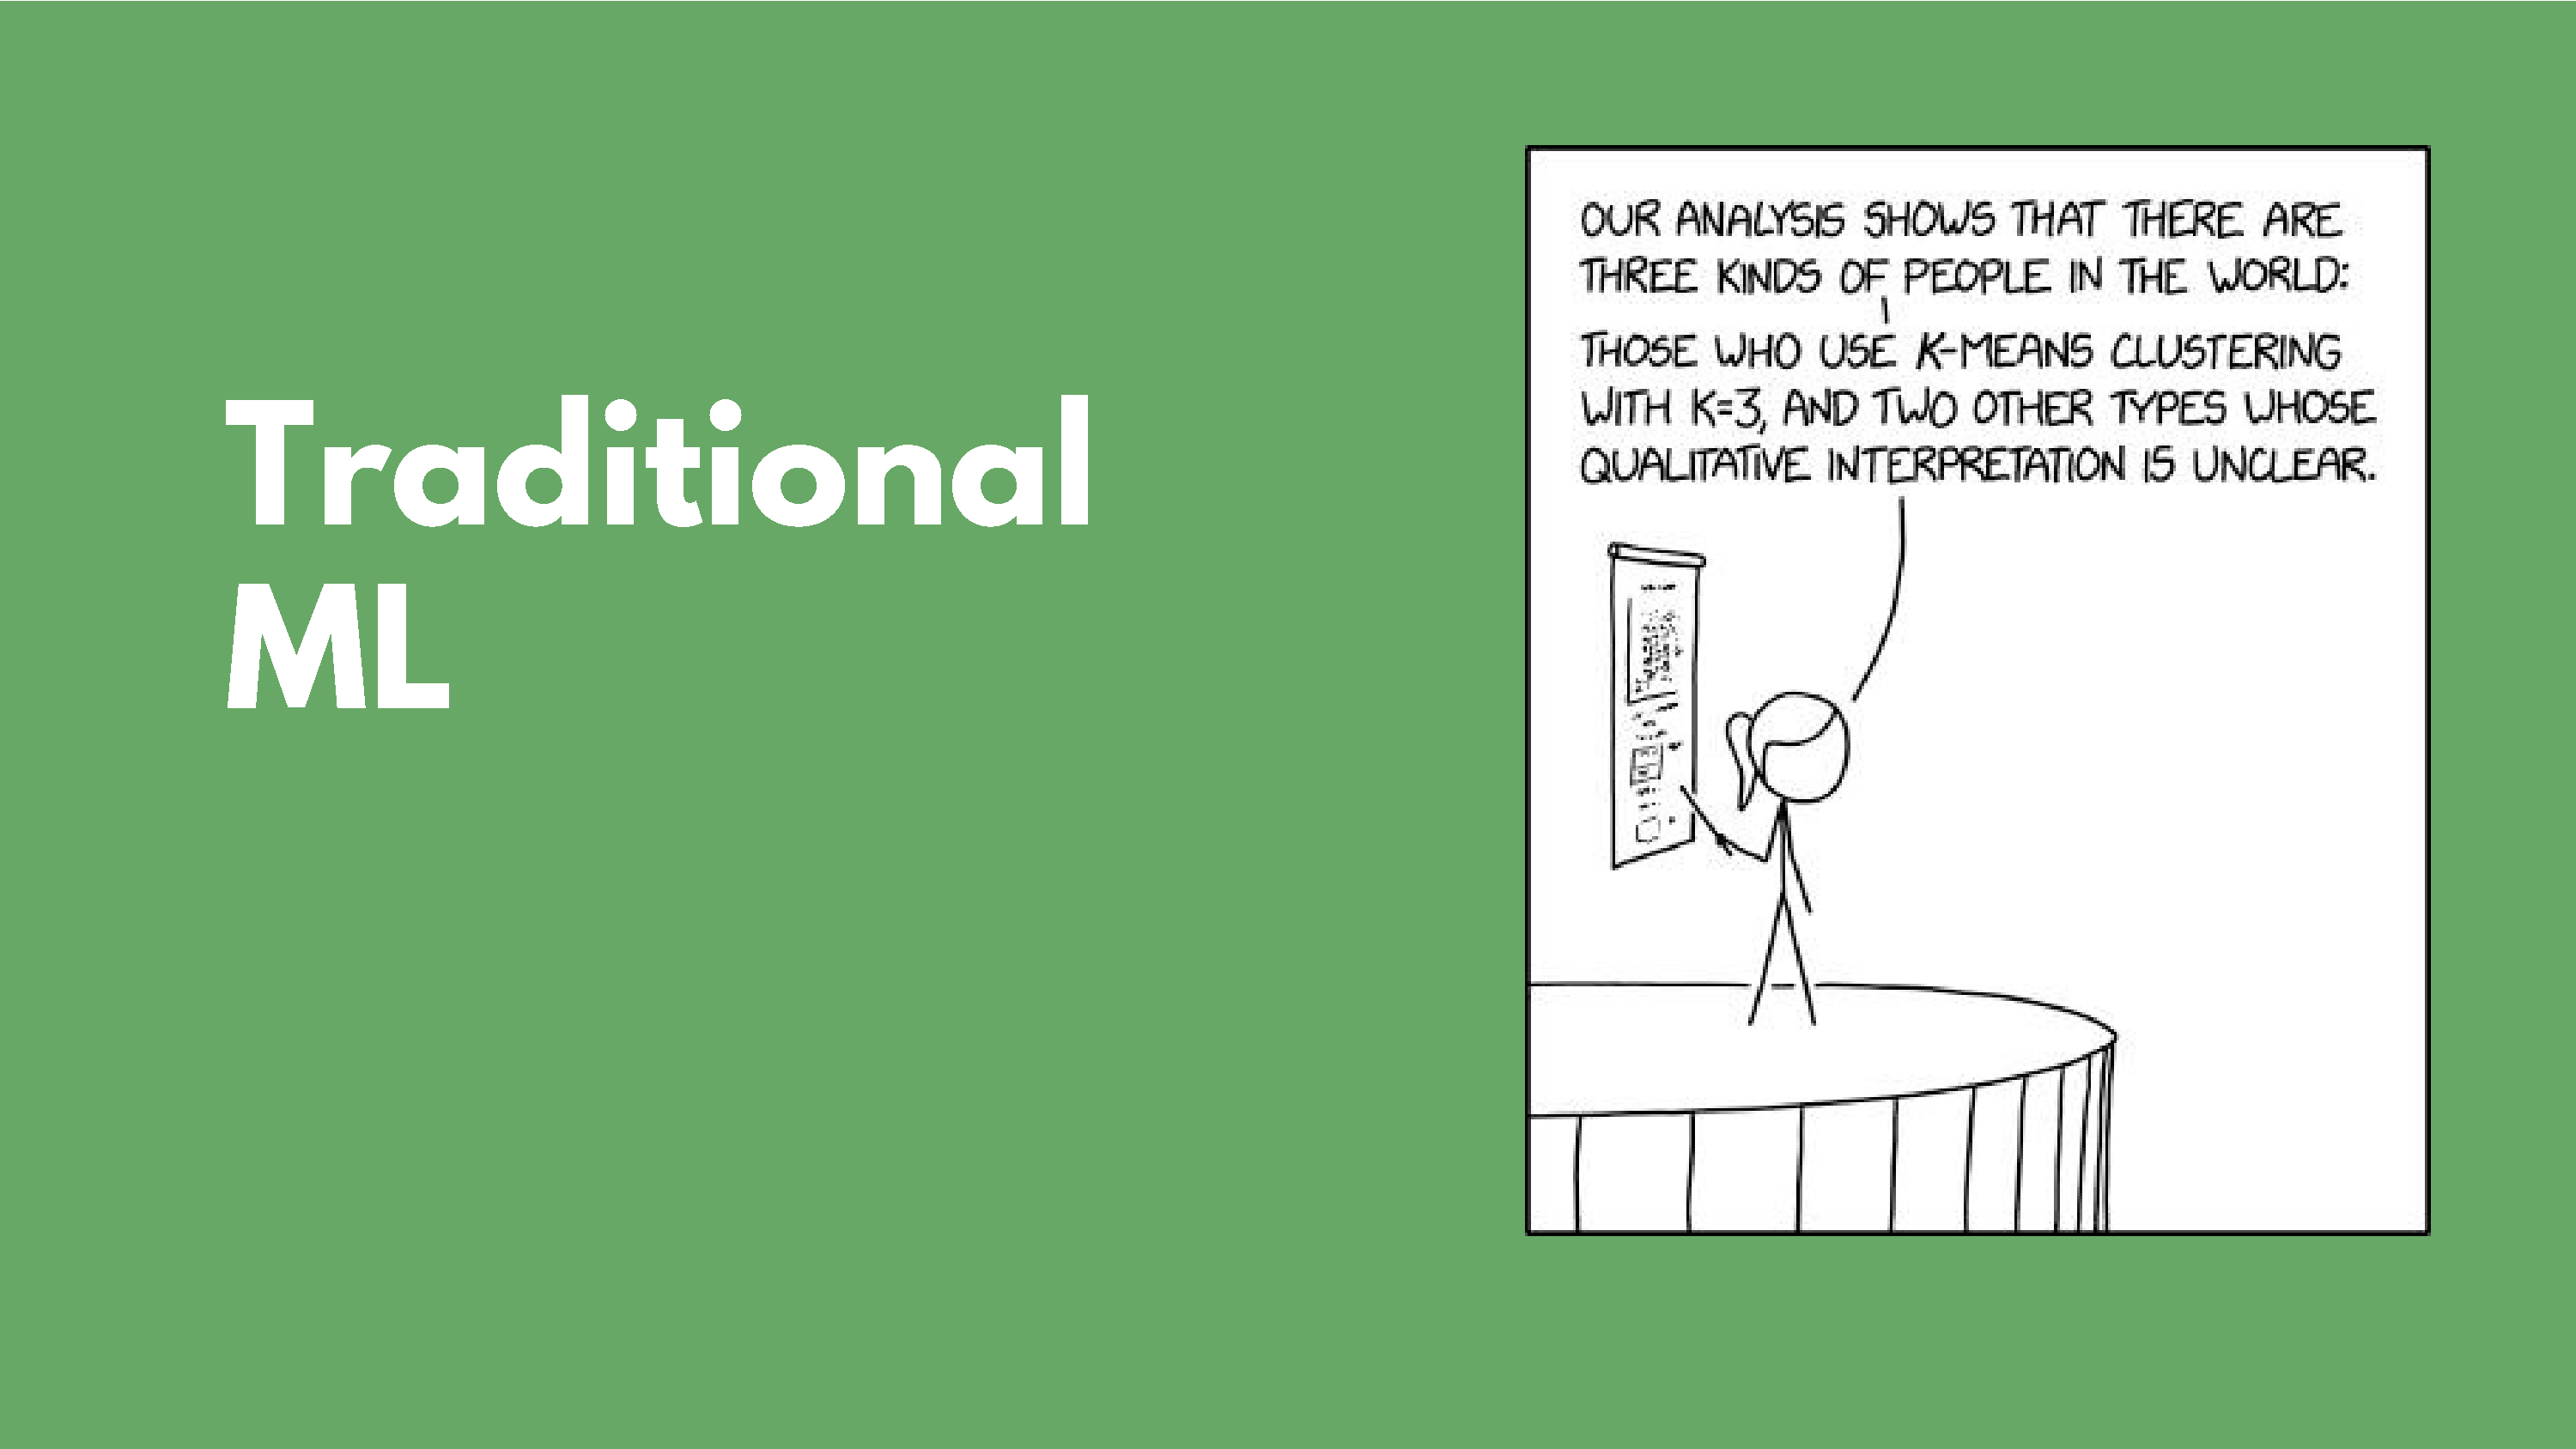
\includegraphics[height=\paperheight,width=\paperwidth]{images/tradML.pdf}};
}

\begin{frame}
\end{frame}

\usebackgroundtemplate{ }
%edit as needed



\begin{frame}{Traditional Machine learning}
The older/traditional way of applying machine learning consisted of the following steps:
	\begin{enumerate}[$\bullet$]
		\item \textbf{Feature Extraction}: Features which can be used to discriminate between classes is captured. This step usually requires in-field knowledge about the problem.\pause
		\item \textbf{Model Selection}: A model is selected which trains on the extracted features. Ensable methods can be used to boost performance\pause
		\item \textbf{Cross-validation/Tested}: The model is tested/cross-validated on with held data
	\end{enumerate}
\end{frame}

\begin{frame}{Problems with the traditional approach}
	  \begin{enumerate}[$\bullet$]
		  \item \textbf{Feature Extraction}: This step requires in-field knowledge. It is very difficult to study  a whole new branch of knowledge for a single problem.\pause
		  \item \textbf{Amount of Data}: In the current era, the amount of data sometimes is simply so large that meaningful features are hard to extract \pause
		  \item \textbf{Unorganized Data}: Feature extraction is hard in unorganized data (such as a literary works).
	  \end{enumerate}
  \end{frame}

  \usebackgroundtemplate{%             declare it
  \tikz[overlay,remember picture] \node[opacity=1, at=(current page.center)] {
	 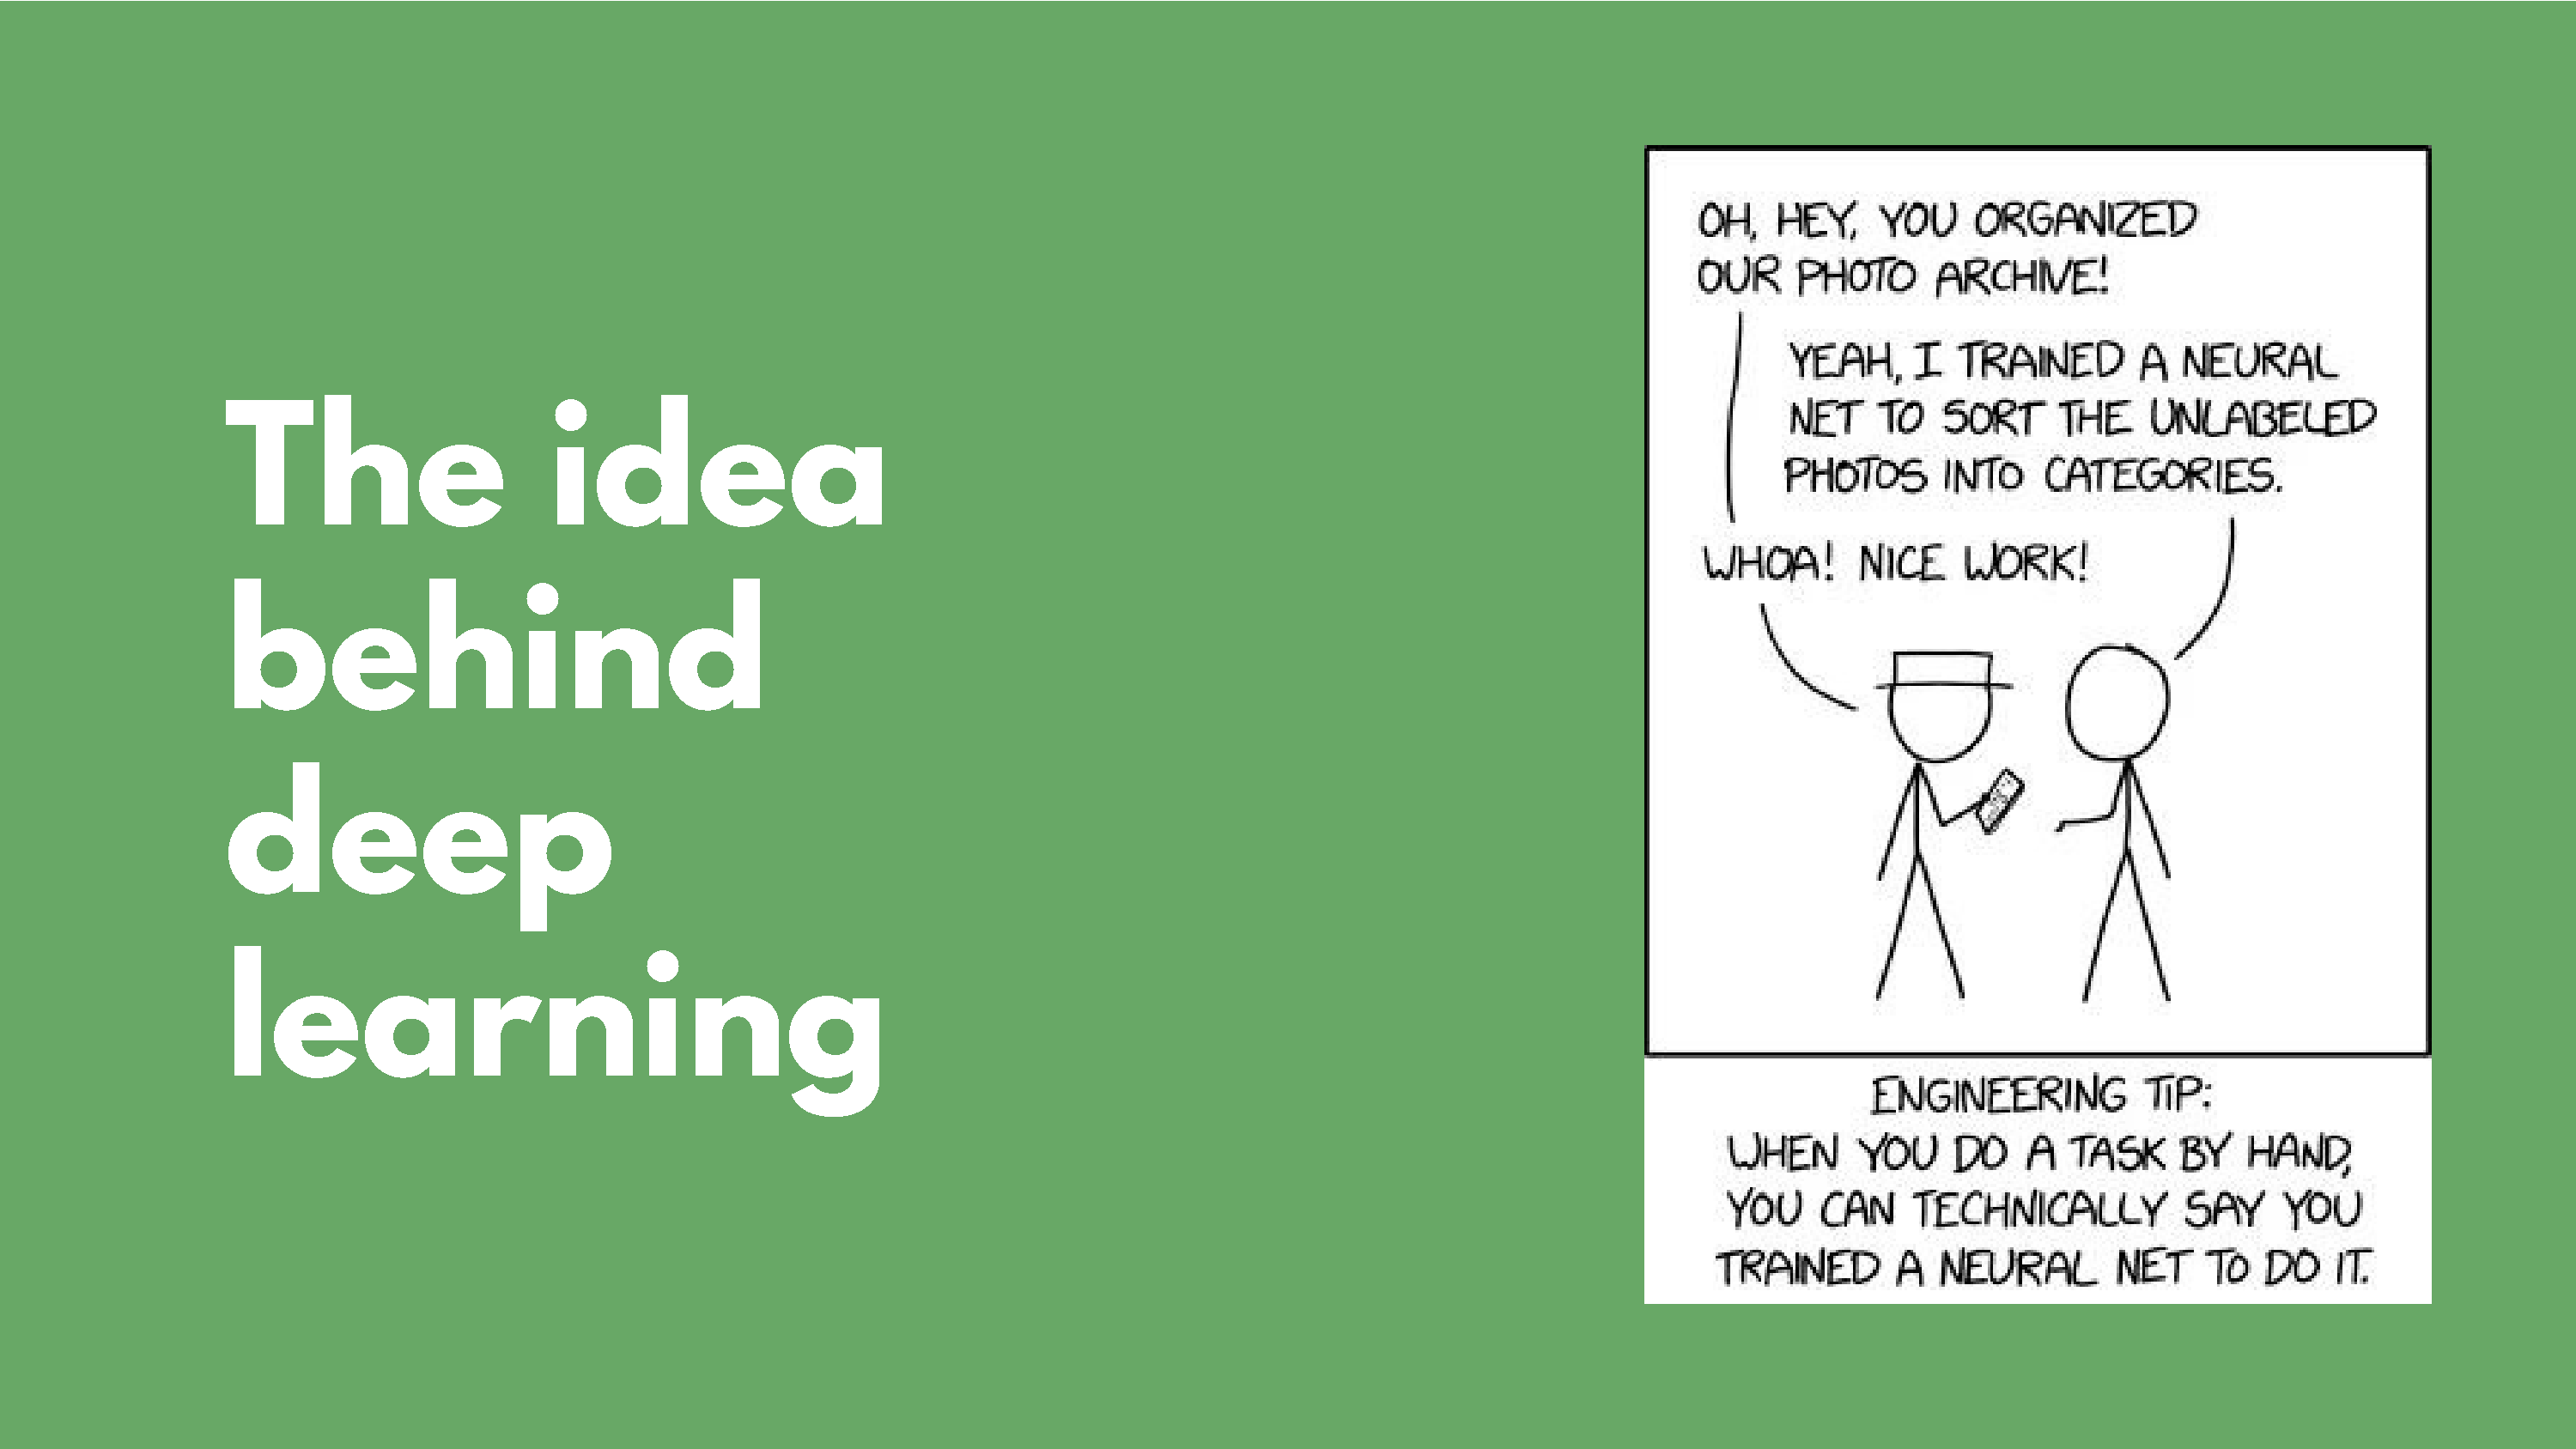
\includegraphics[height=\paperheight,width=\paperwidth]{images/idea_ddepl.pdf}};
  }

  \begin{frame}
  \end{frame}

  \usebackgroundtemplate{ }
  %edit as needed

\begin{frame}{Ideas behind a neural network}
\begin{enumerate}[$\bullet$]
	\item \textbf{Pattern recognition}: Almost all the problems with traditional Ml lies in proper feature selection. We now take a different approach: We train the machine to learn what the necessary patterns/features are.\pause
	\item \textbf{Inspiration}: For this task we take inspiration from the best pattern recognizing machine that we know:\pause\textbf{ our brains}.\pause
	\item \textbf{Overview}: We make a perceptron, which is essentially the digital analog of a neuron. We connect multiple neurons together(similar to our brain) and look at what pattern and amount of activation leads to best result.
\end{enumerate}
\end{frame}



\begin{frame}{A practical comparison with traditional ML}
	\begin{columns}[T]
	\begin{column}{0.4\textwidth}
	  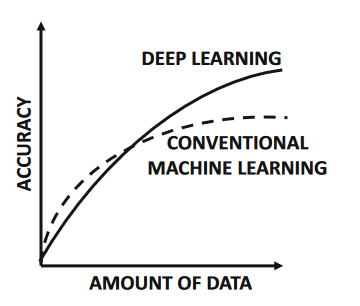
\includegraphics[width=\textwidth]{images/trad vs deep.png}
	  \tiny{\textit{Comparision based on amount of data features.\\ Src: Neural Networks and Deep Learning: A Textbook, Charu C. Aggarwal}}
	\end{column}
	\begin{column}{0.6\textwidth}
	\begin{enumerate}[$\bullet$]
	\item Traditional ML models show better prediction when the amount of features involved is small. Features can be individually engineered and interpreted.\pause
	\item Deep learning models are better when data is unstructured or there are a lot of features which need to be considered. With proper construction and training almost any decision boundaries can be learned.
	\end{enumerate}
	\end{column}
  \end{columns}
\end{frame}

\usebackgroundtemplate{%             declare it
\tikz[overlay,remember picture] \node[opacity=1, at=(current page.center)] {
   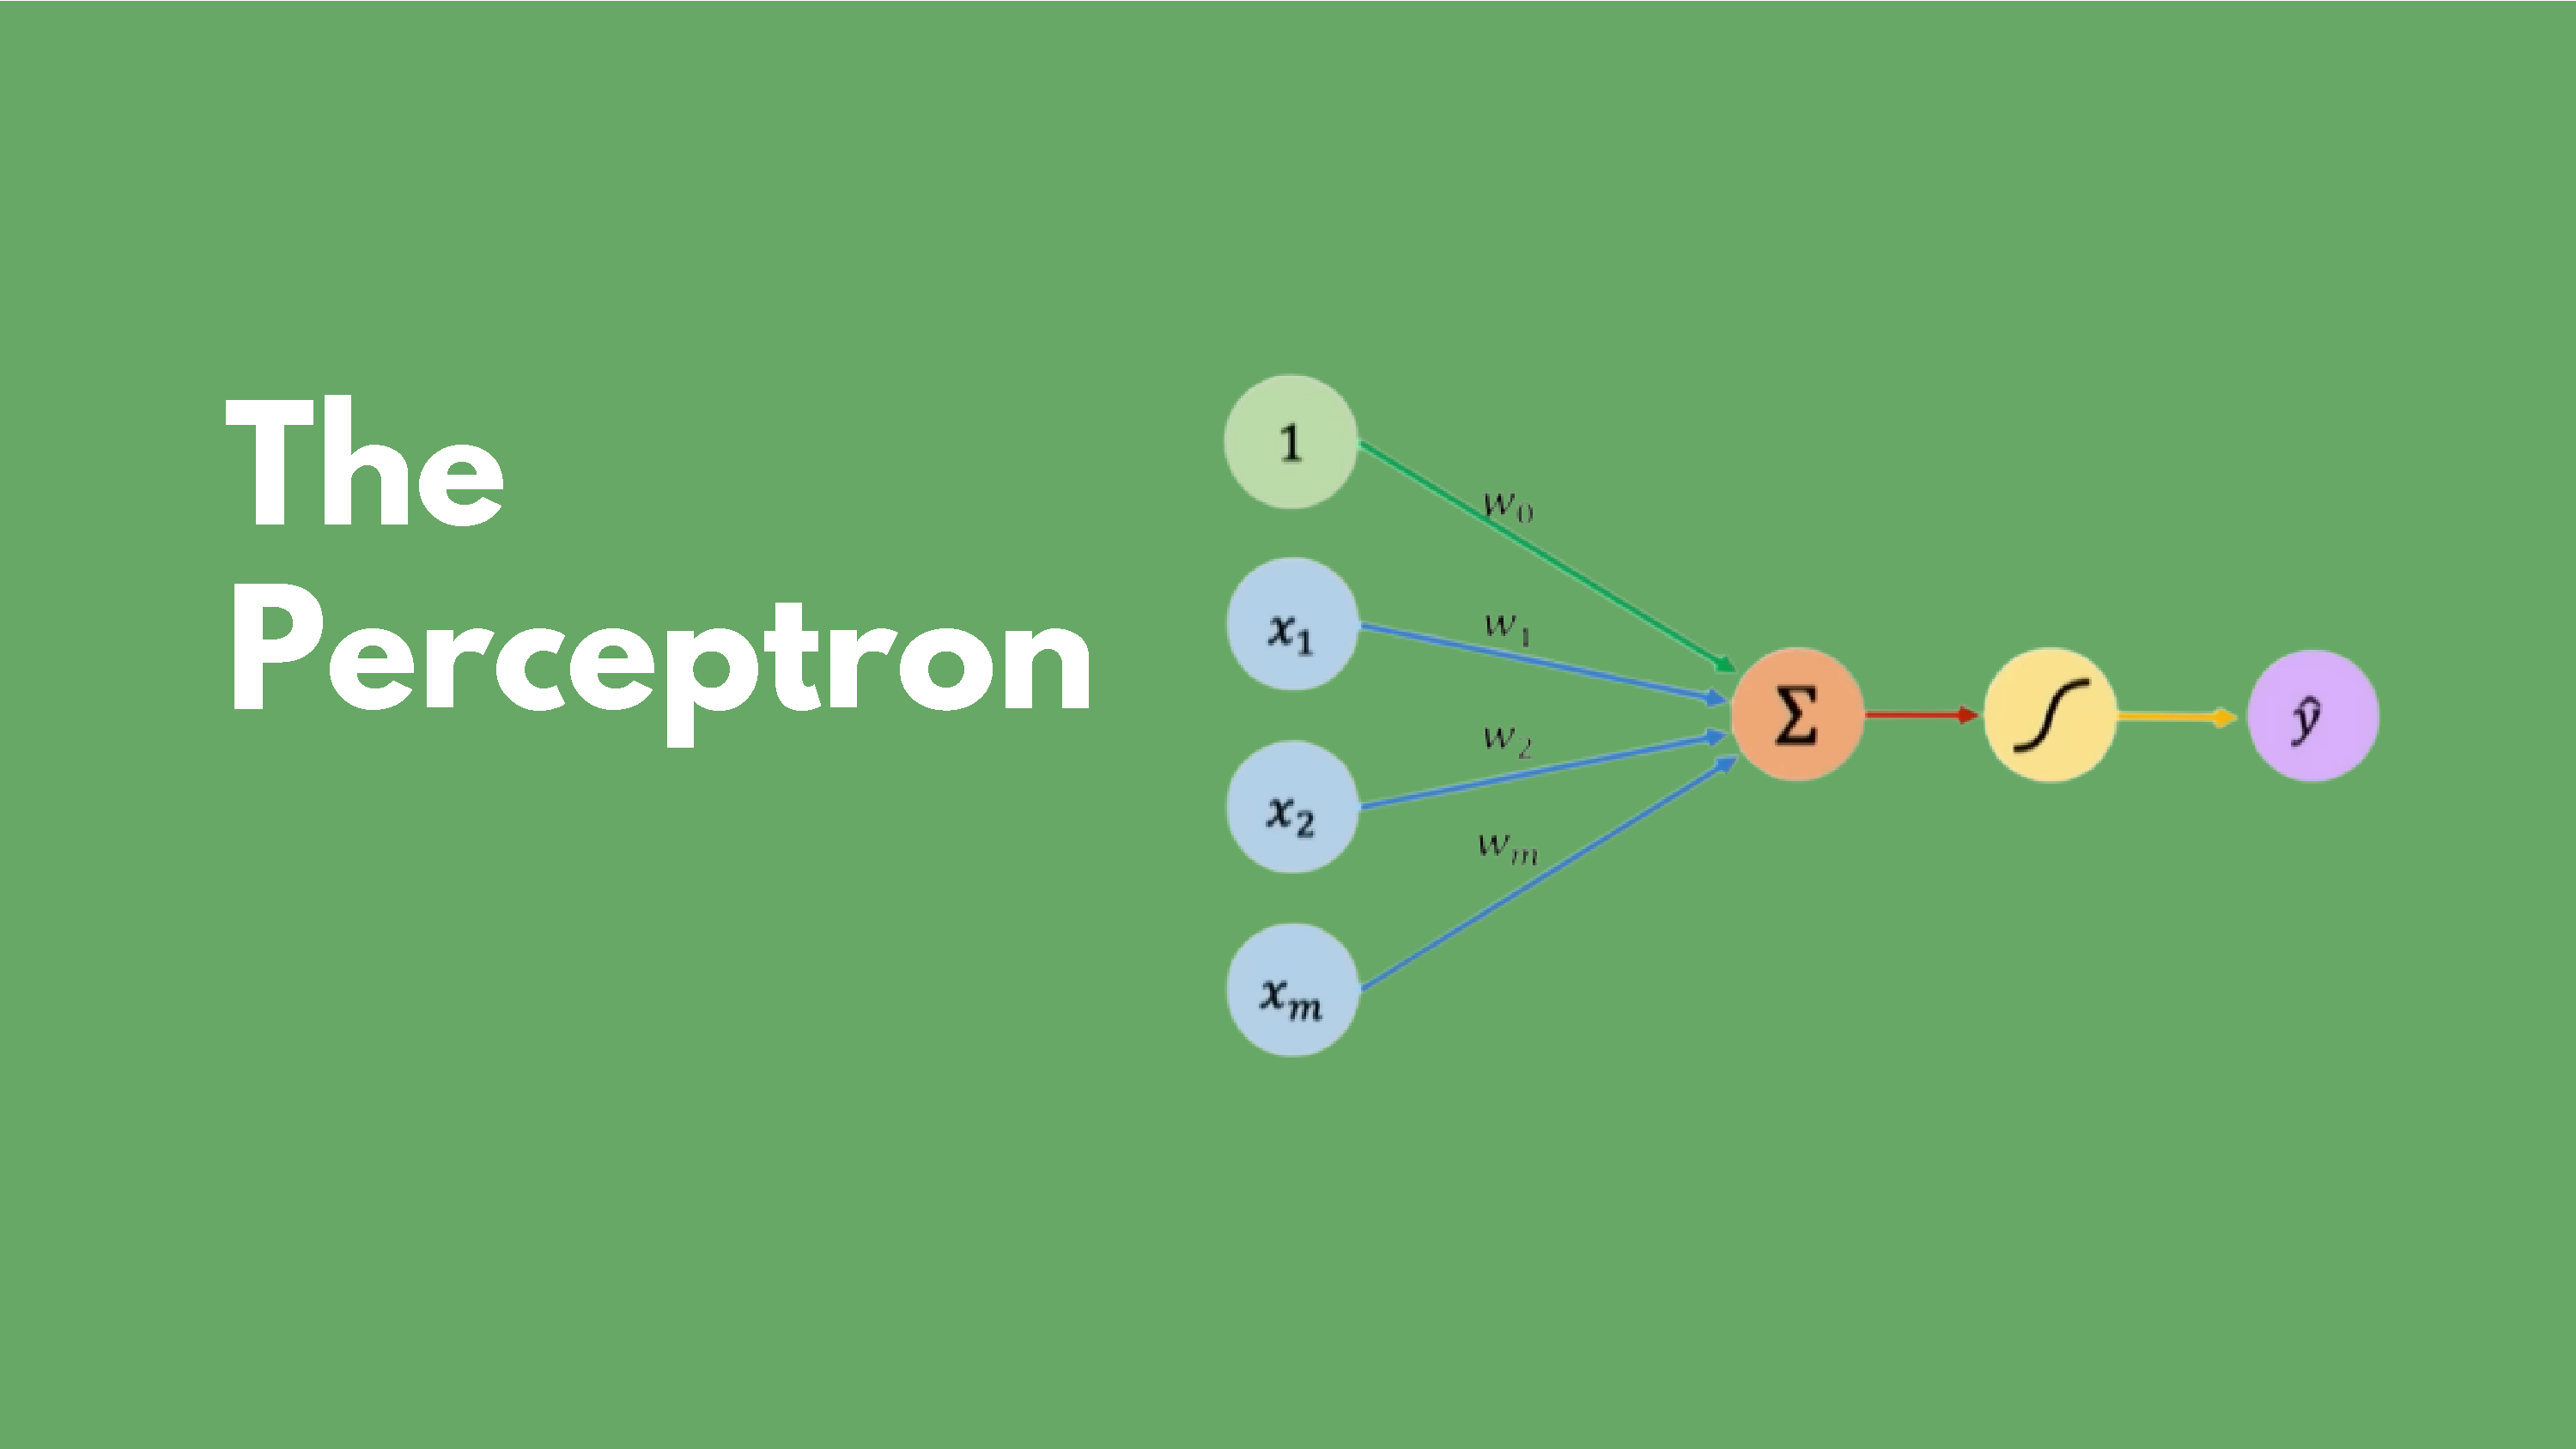
\includegraphics[height=\paperheight,width=\paperwidth]{images/perceptron.pdf}};
}

\begin{frame}
\end{frame}

\usebackgroundtemplate{ }


\begin{frame}{Non-Linearity is the key}
  \begin{columns}[T]
  \begin{column}{0.4\textwidth}
	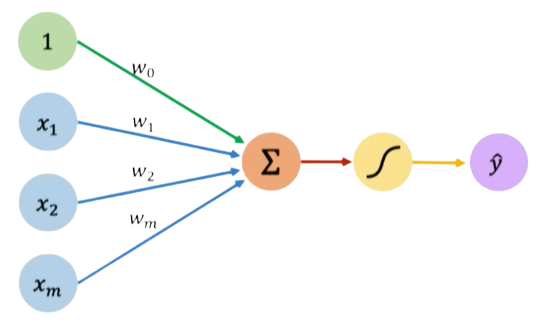
\includegraphics[width=\textwidth]{images/nobg perceptron.png}
	\tiny{\textit{A perceptron\\ Src: MIT Introduction to Deep Learning,6.S191,Lec-1}}
  \end{column}
  \begin{column}{0.6\textwidth}
  \begin{enumerate}[$\bullet$]
  \item The idea behind a perceptron is that a perceptron will give a high value as output when it recognises a certain feature.\pause
  \item Mathematically for an input vector $X$ it outputs $\hat{Y}=\sigma(W^TX+b_0)$ \pause
  \item Multiple perceptrons are wired together(again, much like our brain) to identify richer features.\pause
  \item At the very core, Machine Learning works by constructing proper decision boundaries.\pause
  \item A very simple calculation shows if $\sigma$ is linear then the decision boundary is also linear. It therefore makes sense to use non-linear $\sigma$.
  \end{enumerate}
  \end{column}
\end{columns}
\end{frame}


\begin{frame}{Non-Linearity is the key}
  \begin{columns}[T]
  \begin{column}{0.4\textwidth}
	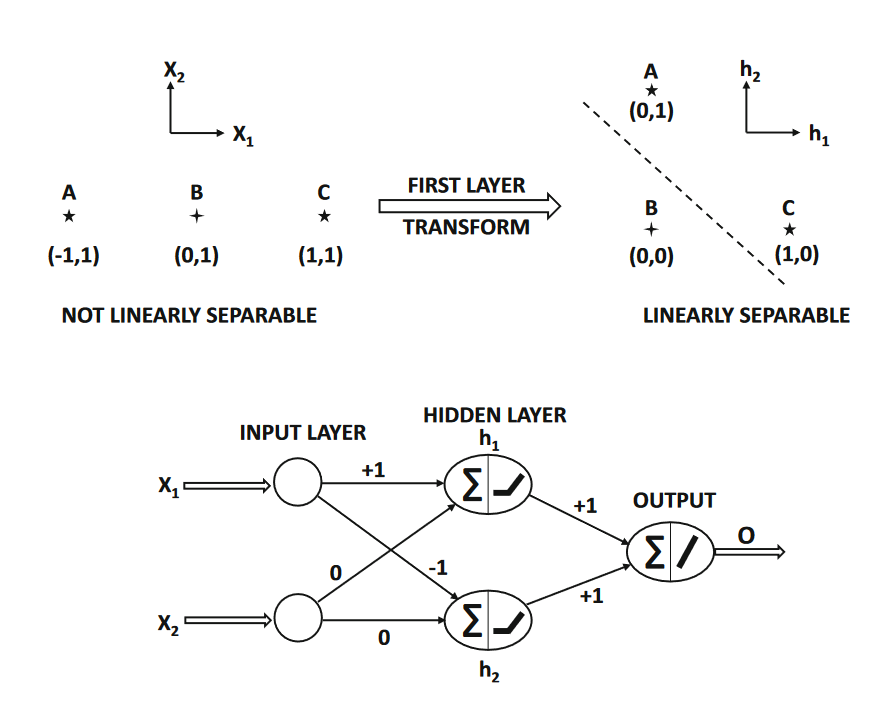
\includegraphics[width=\textwidth]{images/non-linearity.png}
	\tiny{\textit{Non-linearity in action\\ Src: Neural Networks and Deep Learning: A Textbook, Charu C. Aggarwal}}
  \end{column}
  \begin{column}{0.6\textwidth}
  \begin{enumerate}[$\bullet$]
  \item As shown in the figure on left, classes which can't be separated by linear boundaries can be separated by non-linear functions.(Think SVM but the kernals are learned.)\pause
  \item It can be theoretically shown that almost all boundary function can be separated by a 2 layered neural network.
  \end{enumerate}
  \end{column}
\end{columns}
\end{frame}



\begin{frame}{Increasing depth}
  \begin{columns}[T]
  \begin{column}{0.4\textwidth}
	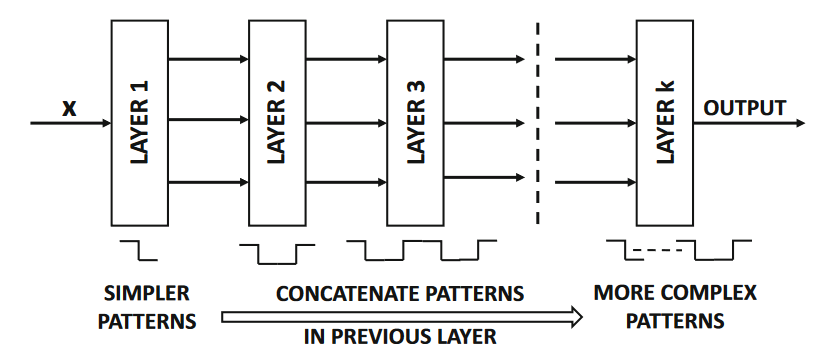
\includegraphics[width=\textwidth]{images/depth.png}
	\tiny{\textit{Why is depth needed\\ Src: Neural Networks and Deep Learning: A Textbook, Charu C. Aggarwal}}
  \end{column}
  \begin{column}{0.6\textwidth}
  \begin{enumerate}[$\bullet$]
  \item While a single hidden layer is enough, making a deep neural network allows us to have more complex decision boundaries with relatively less number of nodes\pause
  \item It should be noted how non-linearity discussed above plays an important role: Irrespective of number of layers, composition of linear functions is linear. On the other hand compositions of non-linear function can lead to richer families of functions. (\textit{Ref: https://www.desmos.com/calculator/m645ggyl2i})
  \end{enumerate}
  \end{column}
\end{columns}
\end{frame}



usebackgroundtemplate{%             declare it
\tikz[overlay,remember picture] \node[opacity=1, at=(current page.center)] {
   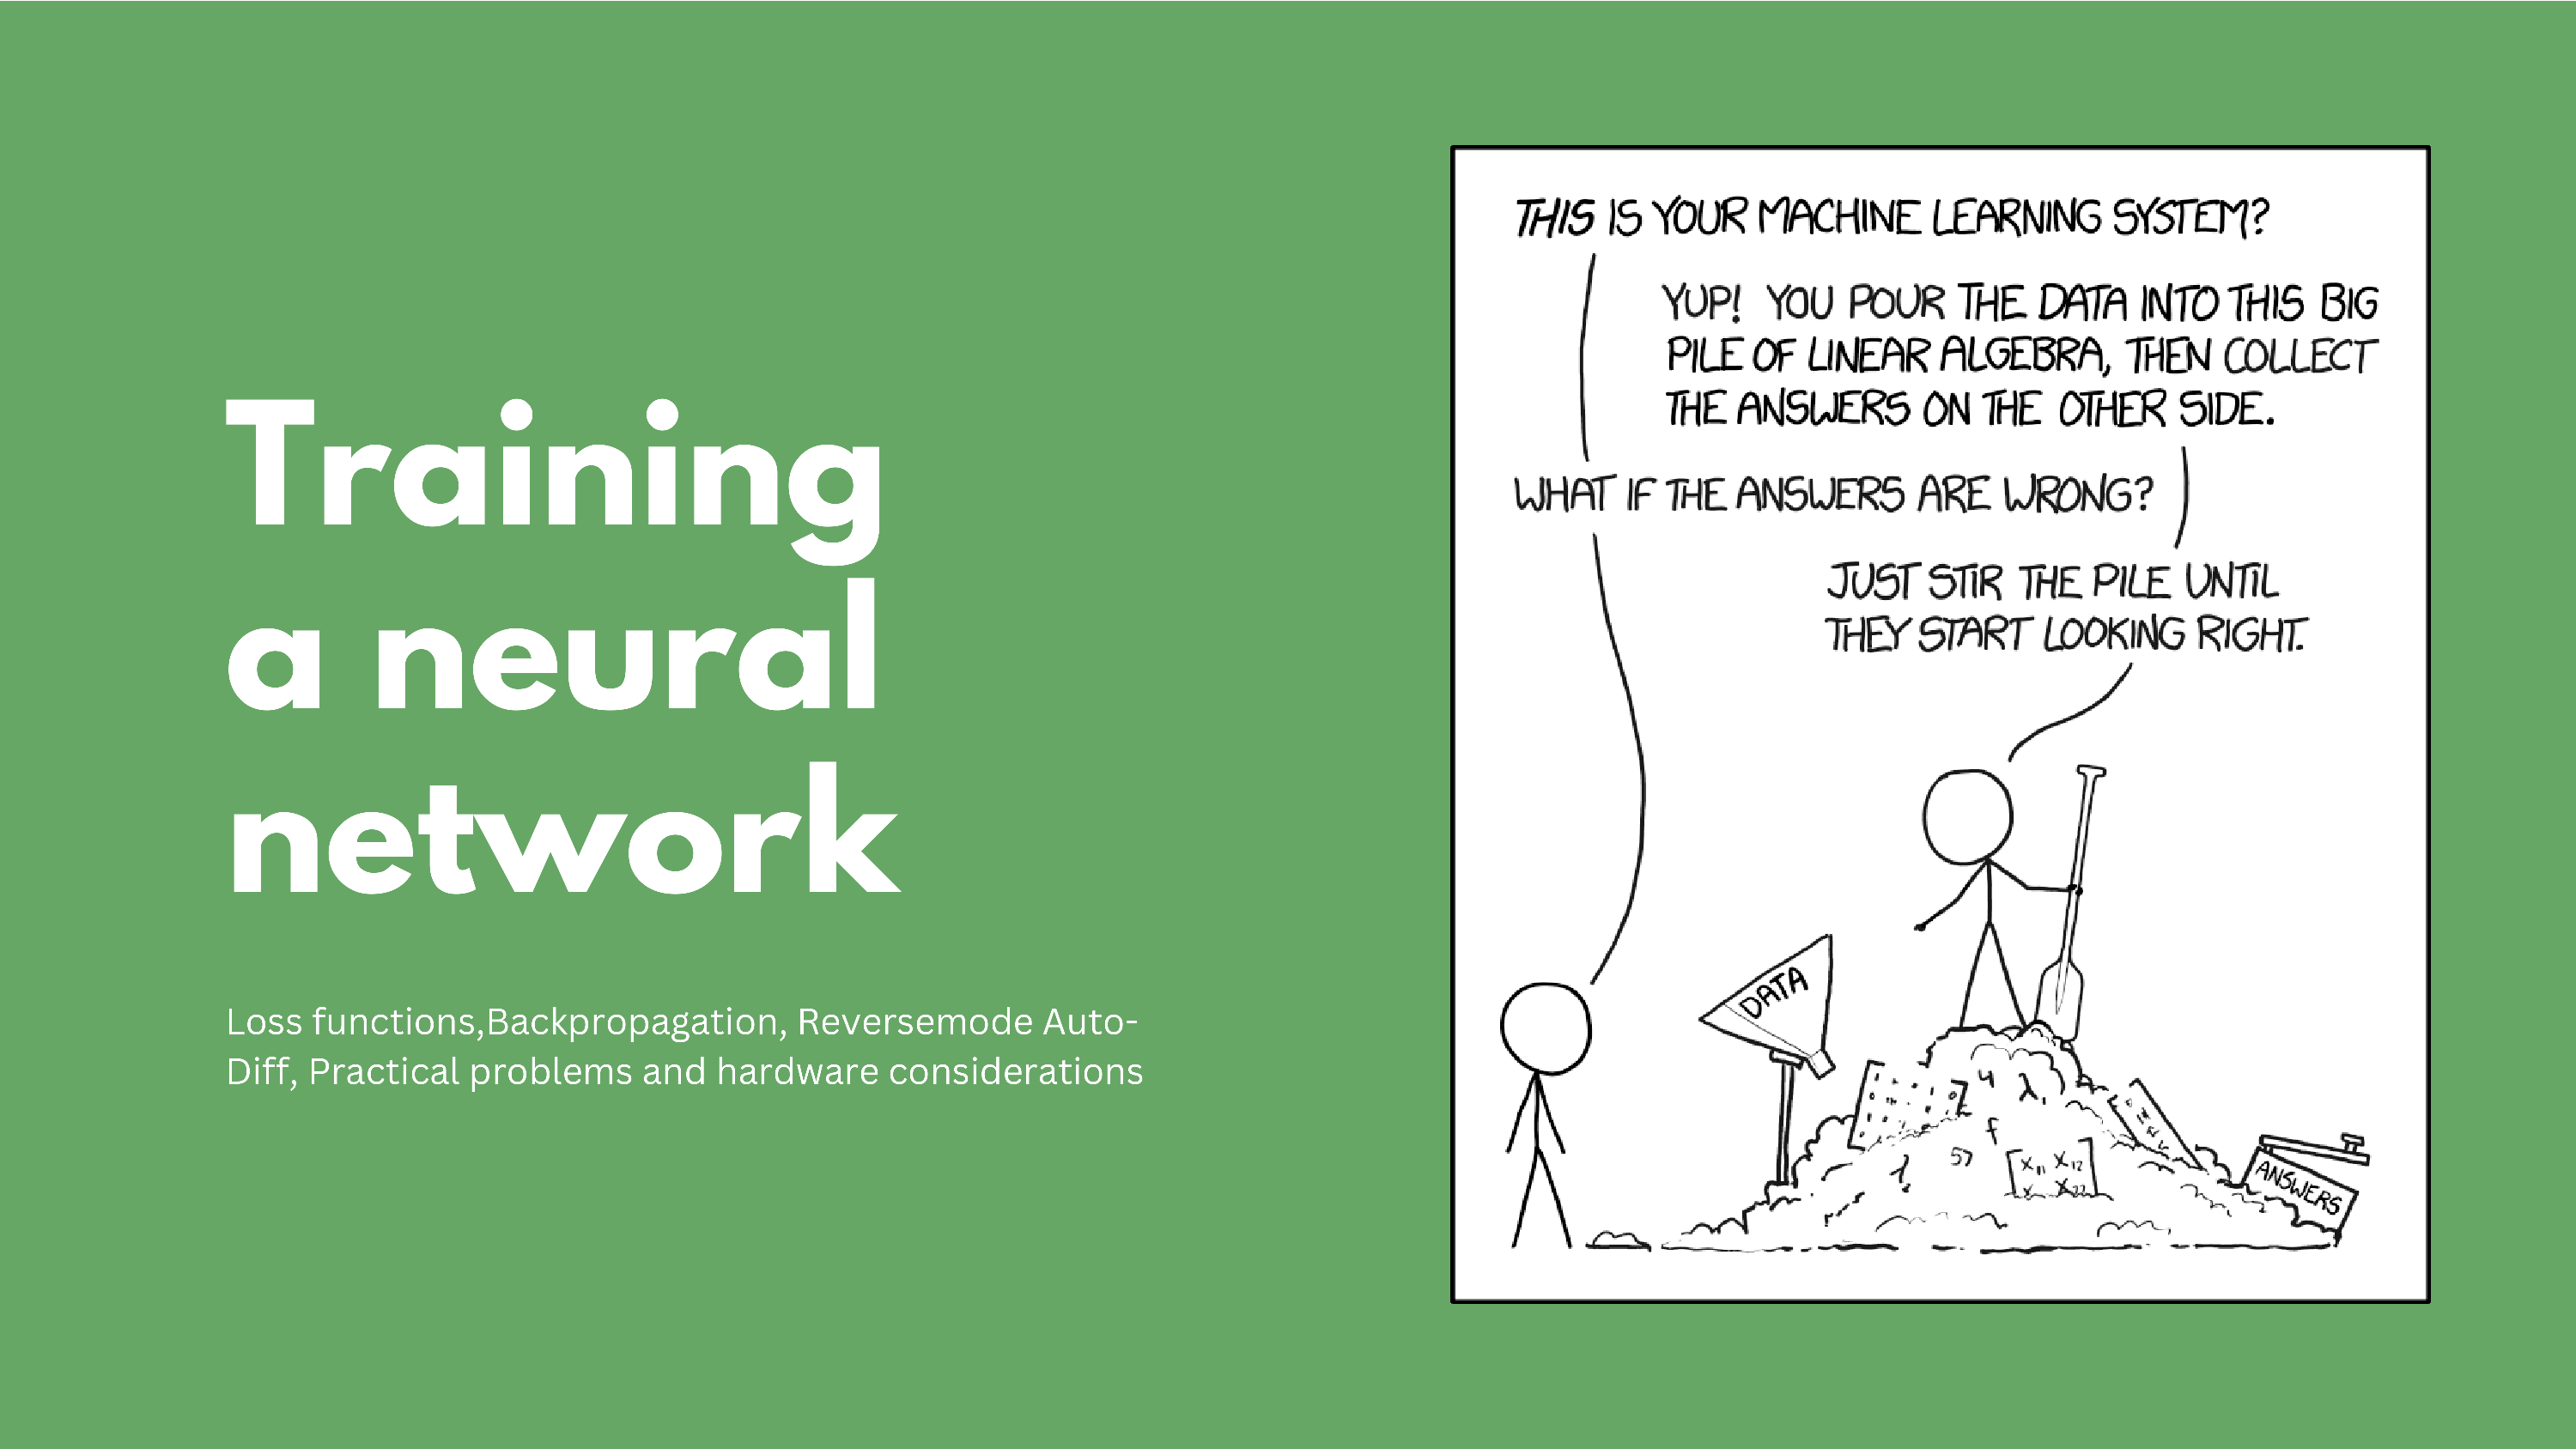
\includegraphics[height=\paperheight,width=\paperwidth]{images/training.pdf}};
}
\begin{frame}
\end{frame}

\usebackgroundtemplate{ }

\begin{frame}{Loss Function}
  \begin{columns}[T]
  \begin{column}{0.4\textwidth}
	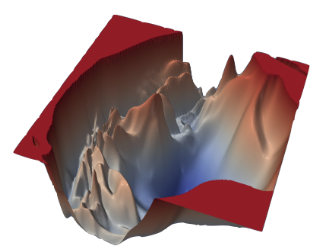
\includegraphics[width=\textwidth]{images/resnet110-noskip-loss.png}
	\tiny{\textit{A slice of the loss landscape of resnet-110 with no skip connections\\ Src: Visualizing the Loss Landscape of Neural Nets, Hao Li, Zheng Xu, Gavin Taylor, Christoph Studer, Tom Goldstein}}
  \end{column}
  \begin{column}{0.6\textwidth}
  \begin{enumerate}[$\bullet$]
  \item We wish to calculate weights $w_i,1\leq i\leq n$ so that the predicted values $\hat{Y}$ are as close as possible(to an extent) to the actual values $Y$.\pause To do this we try to minimize a loss function $\mathcal{L}(\{\hat Y_i\},\{Y_i\})$\pause
  \item Common choices of $\mathcal L$ include MSE for continuous variables and cross-loss entropy for categorical variables.
  \end{enumerate}
  \end{column}
\end{columns}
\end{frame}


\begin{frame}{Gradient descent}
  \begin{columns}[T]
  \begin{column}{0.4\textwidth}
	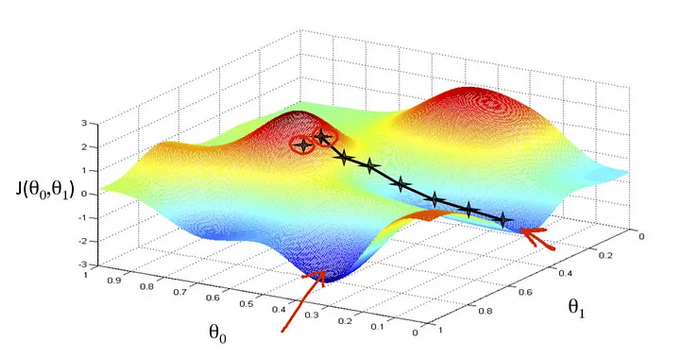
\includegraphics[width=\textwidth]{images/grad-desc.png}
	\tiny{\textit{Gradient descent\\ Src: https://towardsdatascience.com/an-intuitive-explanation-of-gradient-descent-83adf68c9c33}}
  \end{column}
  \begin{column}{0.6\textwidth}
  \begin{enumerate}[$\bullet$]
  \item To find the correct set of weights, we use a greedy approach. We check the surrounding landscape of the weight(i.e. calculate the gradient) and take a step in the direction which leads to maximum decrease in $\mathcal L$. Mathematically, we have:
  $$w_i=wi-\eta \frac{\partial \mathcal L}{\partial w_i}$$\pause
  \item $\eta$ is known as the learning rate.
  \end{enumerate}
  \end{column}
\end{columns}
\end{frame}


\begin{frame}{Learning Rate}
  \begin{columns}[T]
  \begin{column}{0.4\textwidth}
	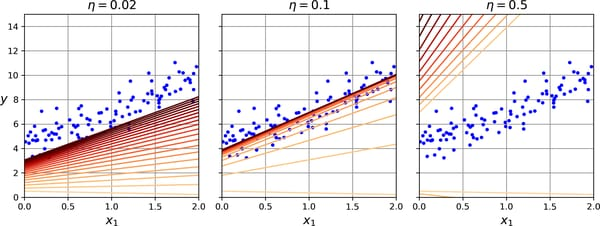
\includegraphics[width=1.1\textwidth]{images/learning rate.jpeg}
	\tiny{\textit{Variations in learning rates\\ Src: Hands-On Machine Learning with Scikit-Learn, Keras, and TensorFlow  Concepts, Tools, and Techniques to Build Intelligent Systems-O'Reilly Media, Inc, Aurélien Géron }}
  \end{column}
  \begin{column}{0.6\textwidth}
  \begin{enumerate}[$\bullet$]
  \item Fixing $\eta$ is quite tricky.\pause
  \item If $\eta$ is small we get stuck at local minima\pause
  \item If $\eta$ is large we overshoot our targets and never converge.
  \item The best way to do things is to use a adaptive learn rate. Some methods(parametric, non-parametric and hybrid are discussed later, once we cover backpropagation)
  \end{enumerate}
  \end{column}
\end{columns}
\end{frame}


\begin{frame}{Backpropagation}
  Consider a neural network to be an acyclic directed graph
  \begin{enumerate}[$\bullet$]
  \item We want to calculate the partial derivative of a node with respect to the other.\pause
  \item The way to do this is to use the chain rule\pause
  \item When we use the chain rule, we sum the partial derivative along all the paths joining the two nodes
  \item It is easy to see that the computation needed explodes as the depth increases
  \item The way to navigate this problem is to use dynamic programming.
  \end{enumerate}
\end{frame}

\begin{frame}
\begin{center}


\tikzset{every picture/.style={line width=0.75pt}} %set default line width to 0.75pt

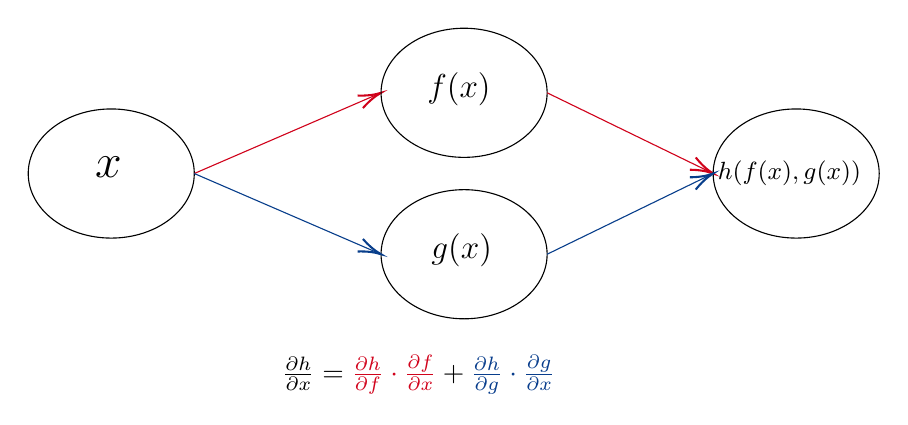
\begin{tikzpicture}[x=0.75pt,y=0.75pt,yscale=-1,xscale=1]
%uncomment if require: \path (0,300); %set diagram left start at 0, and has height of 300

%Shape: Ellipse [id:dp3367595598760599]
\draw   (0,70) .. controls (0,52.82) and (17.91,38.89) .. (40,38.89) .. controls (62.09,38.89) and (80,52.82) .. (80,70) .. controls (80,87.18) and (62.09,101.11) .. (40,101.11) .. controls (17.91,101.11) and (0,87.18) .. (0,70) -- cycle ;
%Straight Lines [id:da39910224852829135]
\draw [color={rgb, 255:red, 208; green, 2; blue, 27 }  ,draw opacity=1 ]   (80,70) -- (168.16,31.9) ;
\draw [shift={(170,31.11)}, rotate = 156.63] [color={rgb, 255:red, 208; green, 2; blue, 27 }  ,draw opacity=1 ][line width=0.75]    (10.93,-3.29) .. controls (6.95,-1.4) and (3.31,-0.3) .. (0,0) .. controls (3.31,0.3) and (6.95,1.4) .. (10.93,3.29)   ;
%Shape: Ellipse [id:dp014340350236969002]
\draw   (170,31.11) .. controls (170,13.93) and (187.91,0) .. (210,0) .. controls (232.09,0) and (250,13.93) .. (250,31.11) .. controls (250,48.29) and (232.09,62.22) .. (210,62.22) .. controls (187.91,62.22) and (170,48.29) .. (170,31.11) -- cycle ;
%Straight Lines [id:da30953970172924394]
\draw [color={rgb, 255:red, 208; green, 2; blue, 27 }  ,draw opacity=1 ]   (250,31.11) -- (328.2,69.13) ;
\draw [shift={(330,70)}, rotate = 205.92] [color={rgb, 255:red, 208; green, 2; blue, 27 }  ,draw opacity=1 ][line width=0.75]    (10.93,-3.29) .. controls (6.95,-1.4) and (3.31,-0.3) .. (0,0) .. controls (3.31,0.3) and (6.95,1.4) .. (10.93,3.29)   ;
%Shape: Ellipse [id:dp1322107562231436]
\draw   (330,70) .. controls (330,52.82) and (347.91,38.89) .. (370,38.89) .. controls (392.09,38.89) and (410,52.82) .. (410,70) .. controls (410,87.18) and (392.09,101.11) .. (370,101.11) .. controls (347.91,101.11) and (330,87.18) .. (330,70) -- cycle ;
%Shape: Ellipse [id:dp6161135526872799]
\draw   (170,108.89) .. controls (170,91.71) and (187.91,77.78) .. (210,77.78) .. controls (232.09,77.78) and (250,91.71) .. (250,108.89) .. controls (250,126.07) and (232.09,140) .. (210,140) .. controls (187.91,140) and (170,126.07) .. (170,108.89) -- cycle ;
%Straight Lines [id:da31403089636099324]
\draw [color={rgb, 255:red, 8; green, 62; blue, 139 }  ,draw opacity=1 ]   (250,108.89) -- (328.2,70.87) ;
\draw [shift={(330,70)}, rotate = 154.08] [color={rgb, 255:red, 8; green, 62; blue, 139 }  ,draw opacity=1 ][line width=0.75]    (10.93,-3.29) .. controls (6.95,-1.4) and (3.31,-0.3) .. (0,0) .. controls (3.31,0.3) and (6.95,1.4) .. (10.93,3.29)   ;
%Straight Lines [id:da9909467052529207]
\draw [color={rgb, 255:red, 8; green, 62; blue, 139 }  ,draw opacity=1 ]   (80,70) -- (168.16,108.1) ;
\draw [shift={(170,108.89)}, rotate = 203.37] [color={rgb, 255:red, 8; green, 62; blue, 139 }  ,draw opacity=1 ][line width=0.75]    (10.93,-3.29) .. controls (6.95,-1.4) and (3.31,-0.3) .. (0,0) .. controls (3.31,0.3) and (6.95,1.4) .. (10.93,3.29)   ;


% Text Node
\draw (31,60.96) node [anchor=north west][inner sep=0.75pt]  [font=\LARGE]  {$x$};
% Text Node
\draw (191,19.96) node [anchor=north west][inner sep=0.75pt]  [font=\large]  {$f( x)$};
% Text Node
\draw (193,97.73) node [anchor=north west][inner sep=0.75pt]  [font=\large]  {$g( x)$};
% Text Node
\draw (331,62.62) node [anchor=north west][inner sep=0.75pt]  [font=\small]  {$h( f( x) ,g( x))$};
% Text Node
\draw (121,156.4) node [anchor=north west][inner sep=0.75pt]    {$\frac{\partial h}{\partial x} =\textcolor[rgb]{0.82,0.01,0.11}{\frac{\partial h}{\partial f} \cdot \frac{\partial f}{\partial x}} +\textcolor[rgb]{0.03,0.24,0.55}{\frac{\partial h}{\partial g} \cdot \frac{\partial g}{\textcolor[rgb]{0.03,0.24,0.55}{\partial x}}}$};


\end{tikzpicture}

\end{center}
\end{frame}
\begin{frame}{Backpropagation}
	Roughly, the alogirithm works as follows:
	\begin{enumerate}[$\bullet$]
	\item Initialize the weights\pause
	\item Calculate $\mathcal{L}$. Note, that this step occurs from the input towards the output and is known as the forward phase.
	\item Calculate gradient. This process occurs from the output towards the input and is known as the backward phase.
	\end{enumerate}
  \end{frame}


  \begin{frame}{Reverse Mode Auto Differentiation}
	\begin{columns}[T]
	\begin{column}{0.8\textwidth}
	\begin{center}
		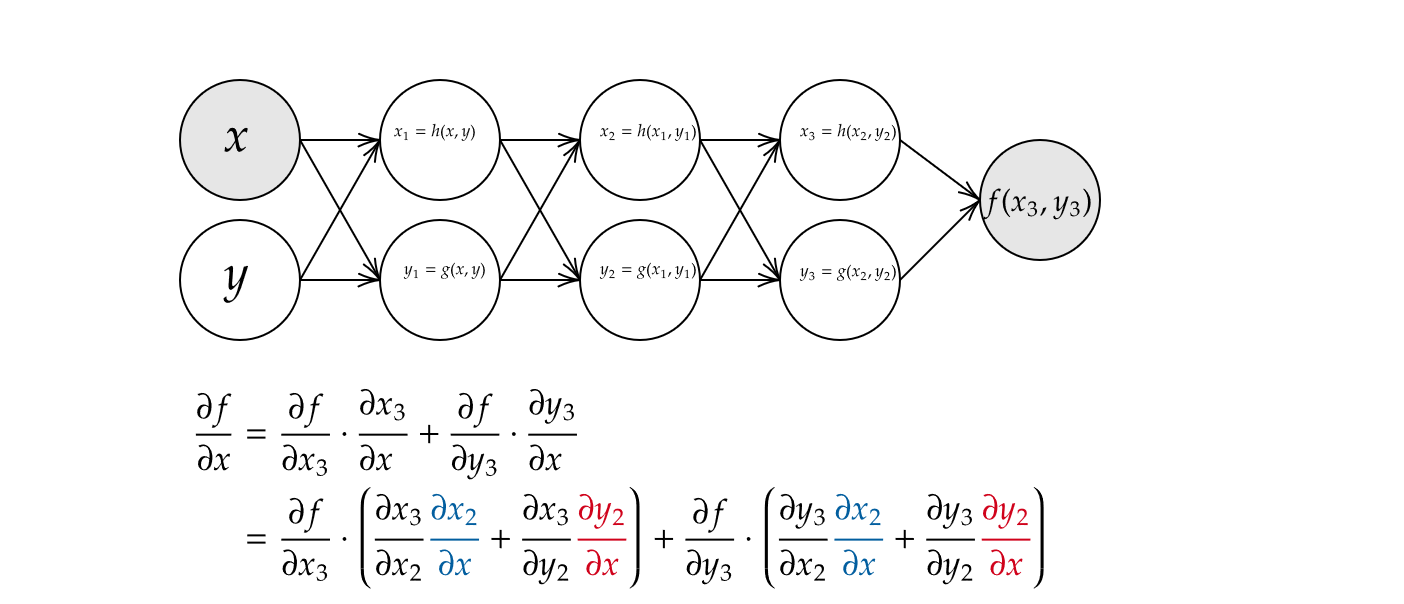
\includegraphics[width=\textwidth]{images/revmodeautodiff.png}
	\end{center}
	\end{column}
	\begin{column}{0.2\textwidth}
	The whole idea relies on the fact that while calculating gradients, parts of the calculation are repeated.
	\end{column}
	\end{columns}
\end{frame}

\begin{frame}{Reverse Mode Auto Differentiation}
\begin{columns}[T]
\begin{column}{0.7\textwidth}
\begin{center}
	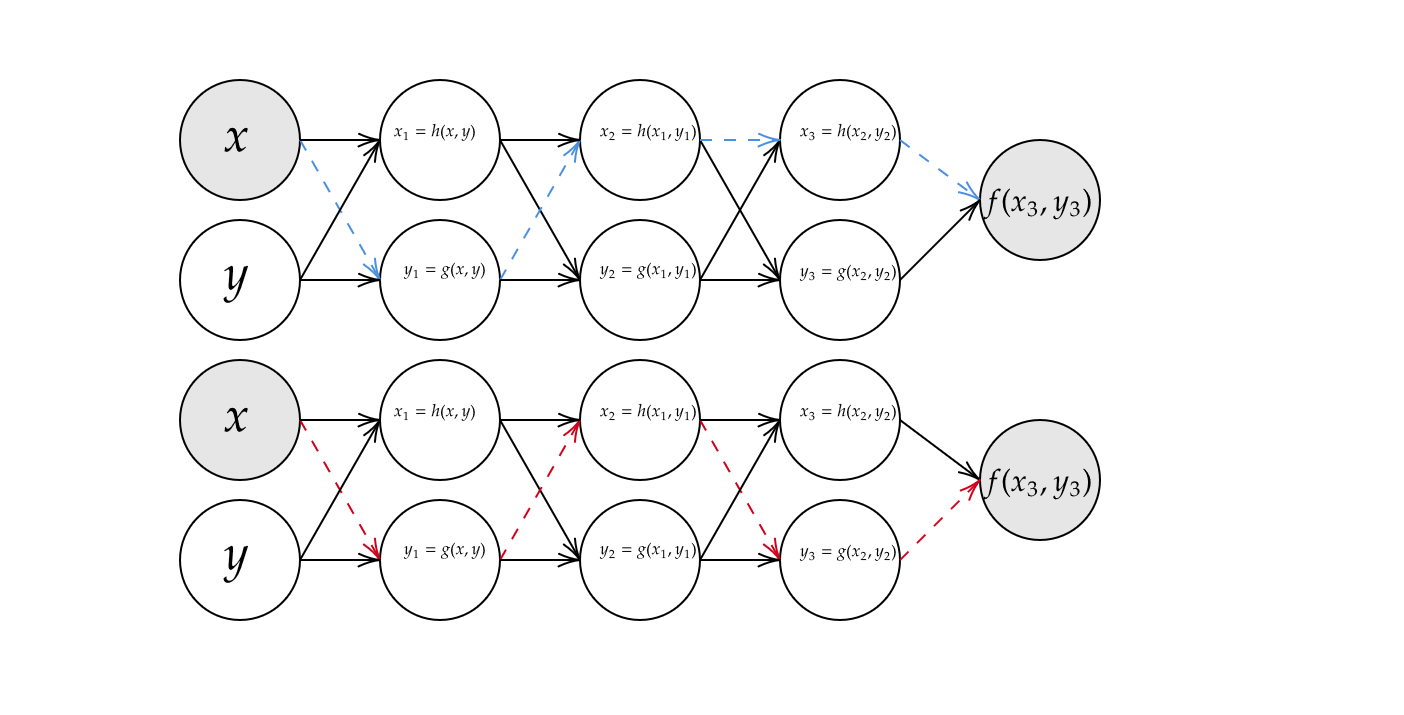
\includegraphics[width=\textwidth]{images/path comp.png}
\end{center}
\end{column}
\begin{column}{0.3\textwidth}
Sum is taken over the product along each path, over all the paths. It is trivial to note that parts of the paths are repeated.\pause In the toy example on the left, the paths are essentially the same, varying only for the second to last node.
\end{column}
\end{columns}
\end{frame}

\begin{frame}{Gradient Descent Statergy-Stochastic Gradient Descent}
	\begin{columns}[T]
	\begin{column}{0.4\textwidth}
	  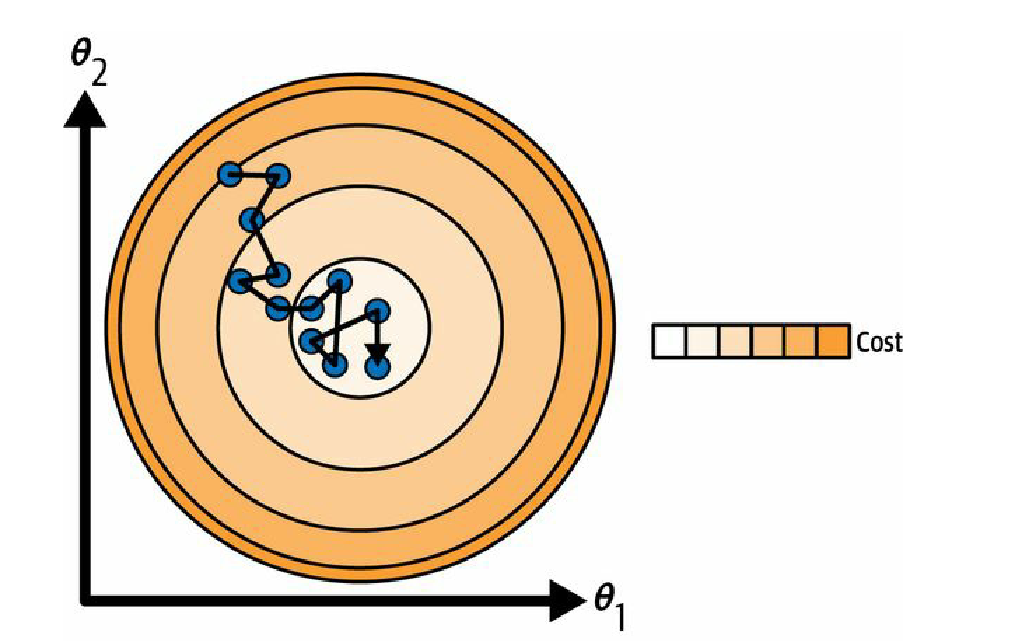
\includegraphics[width=\textwidth]{images/stochastic gradient descent.png}
	  \tiny{\textit{Stochstic Gradient descent\\ Src:Hands-On Machine Learning with Scikit-Learn, Keras, and TensorFlow  Concepts, Tools, and Techniques to Build Intelligent Systems-O'Reilly Media, Inc, Aurélien Géron}}
	\end{column}
	\begin{column}{0.6\textwidth}
	\begin{enumerate}[$\bullet$]
	\item Instead of calculating the total loss, we calculate the loss from a randomly picked sample(or a batch in case of batch gradient descent)\pause
	\item This decreases the computational time.\pause
	\item Think instead of taking slower but confident steps, we take faster but less-confident steps.
	\end{enumerate}
	\end{column}
  \end{columns}
  \end{frame}

  \begin{frame}{Gradient Descent Statergy- Normalization}
	\begin{columns}[T]
        \begin{column}{0.6\textwidth}
        	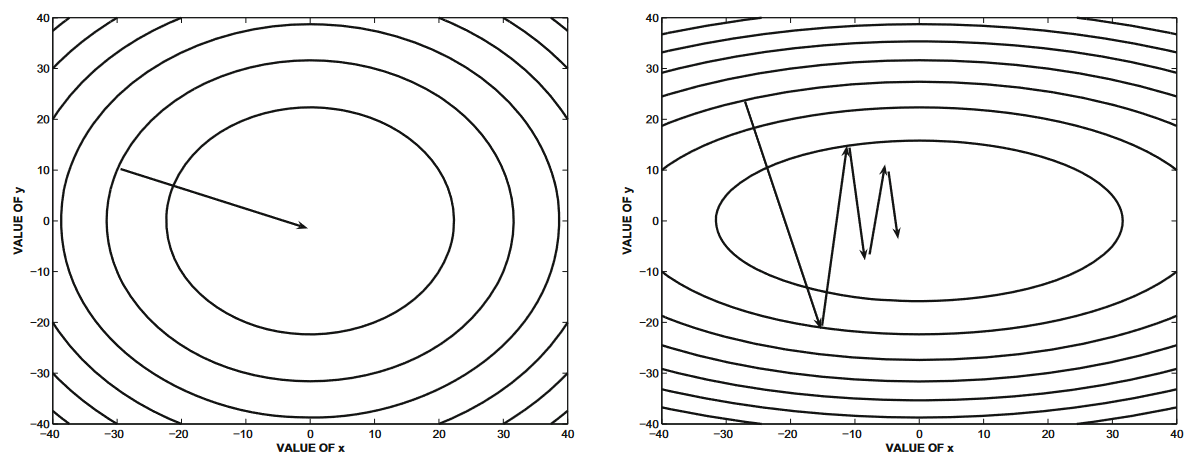
\includegraphics[width=\textwidth]{images/normalise.png}
        	\tiny{\textit{Why normalize?\\ Src:Hands-On Machine Learning with Scikit-Learn, Keras, and TensorFlow  Concepts, Tools, and Techniques to Build Intelligent Systems-O'Reilly Media, Inc, Aurélien Géron}}
        \end{column}
	    \begin{column}{0.4\textwidth}
    	    Normalizing features is a way to make the descent smoother. It essentially lowers the changes in direction orthogonal to the minima.
    	\end{column}
    \end{columns}
\end{frame}


  \begin{frame}{Gradient Descent Statergy- Mommentum}
    \begin{columns}[T]
    \begin{column}{0.4\textwidth}
      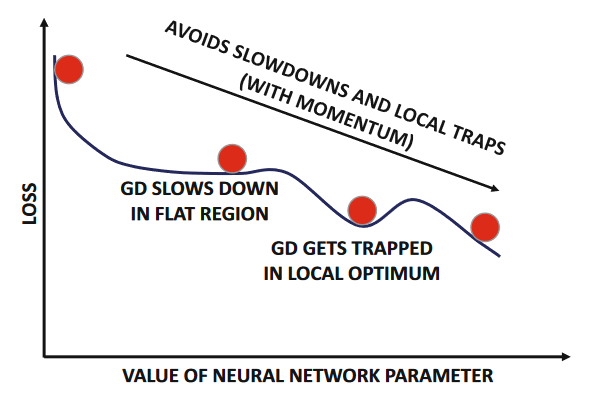
\includegraphics[width=\textwidth]{images/momentum.png}
      \tiny{\textit{Need for momentum\\ Src:Neural Networks and Deep Learning: A Textbook, Charu C. Aggarwal}}
    \end{column}
    \begin{column}{0.6\textwidth}
    \begin{enumerate}[$\bullet$]
    \item A Momentum term might be used in gradient descent where consideration is made for a moving average "velocity" of the descent.\pause
    \item Particularly helps when there are local minimas and flat regions. \pause
    \item  Helps when there is a lot of "zig-zag" but the descent heads in a certain direction.
    \end{enumerate}
    \end{column}
    \end{columns}
\end{frame}


\begin{frame}{Gradient Descent Statergy- Mommentum}
  \begin{columns}[T]
    \begin{column}{0.4\textwidth}
		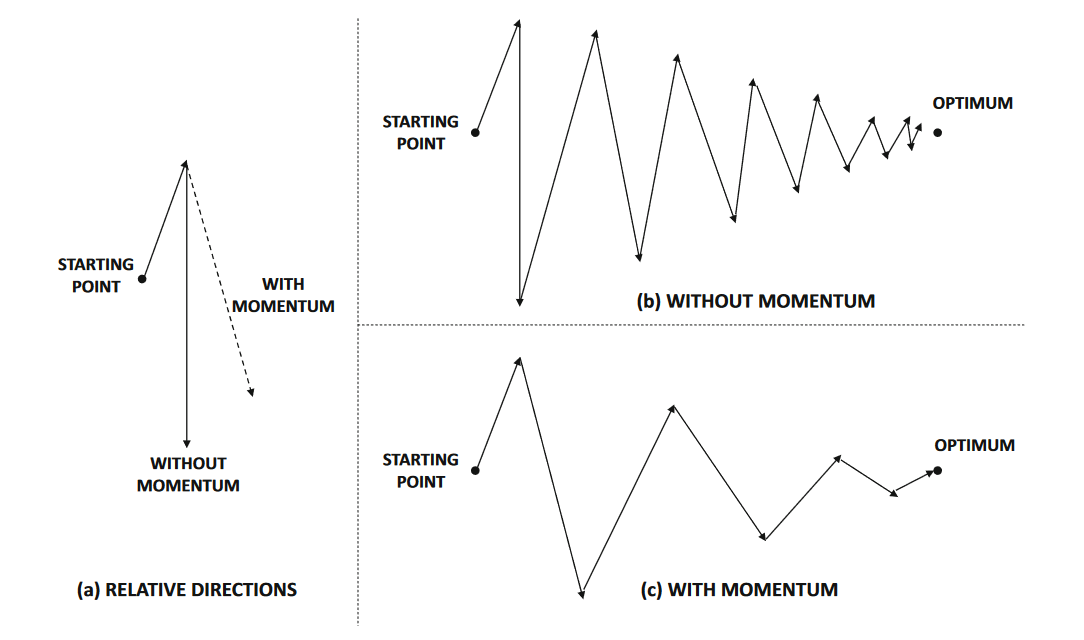
\includegraphics[width=\textwidth]{images/momentum-zigzag.png}
        \tiny{\textit{Need for momentum\\ Src:Neural Networks and Deep Learning: A Textbook, Charu C. Aggarwal}}
    \end{column}
    \begin{column}{0.6\textwidth}
    \begin{enumerate}[$\bullet$]
      \item A Momentum term might be used in gradient descent where consideration is made for a moving average "velocity" of the descent.
      \item Particularly helps when there are local minimas and flat regions.
      \item  Helps when there is a lot of "zig-zag" but the descent heads in a certain direction.
      \end{enumerate}
      \end{column}
      \end{columns}
      \end{frame}

\begin{frame}{Gradient Descent Statergy- Nestov Mommentum}
	\begin{columns}[T]
        \begin{column}{0.4\textwidth}
        	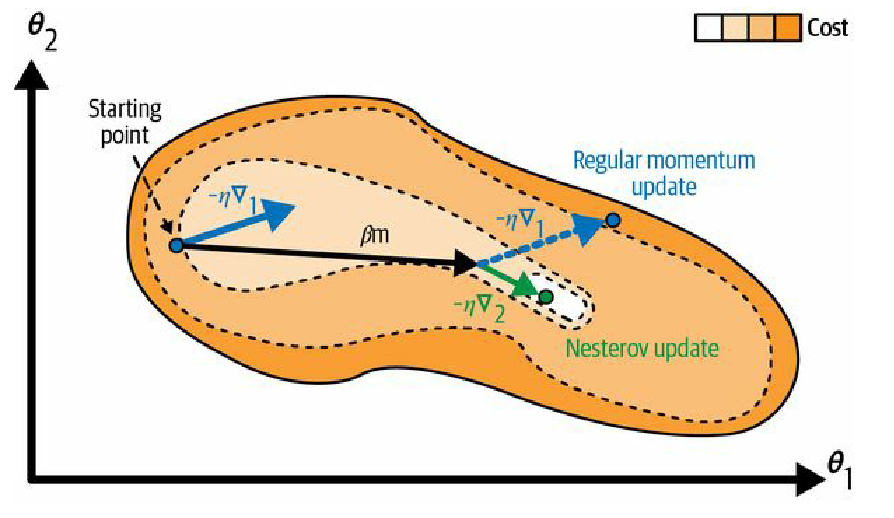
\includegraphics[width=\textwidth]{images/nestov.png}
        	\tiny{\textit{Nestov momentum\\ Src:Hands-On Machine Learning with Scikit-Learn, Keras, and TensorFlow  Concepts, Tools, and Techniques to Build Intelligent Systems-O'Reilly Media, Inc, Aurélien Géron}}
        \end{column}
	    \begin{column}{0.6\textwidth}
    	    \begin{enumerate}[$\bullet$]
        		\item Nestov-momentum is similar to momentum with some scout ahead\pause
        		\item Knowing what's coming up ahead further helps in correcting the direction of descent.
        	\end{enumerate}
    	\end{column}
    \end{columns}
\end{frame}

\begin{frame}{Gradient Descent Statergy- Adaptive Learning Rates}
    \begin{enumerate}[$\bullet$]
		\item We try to let different parameters have different learning rates.\pause
		\item The idea is that parameters with large partial derivatives are often oscillating and
		zigzagging, whereas parameters with small partial derivatives tend to be more consistent
		but move in the same direction.\pause
		\item  Algorithms include AdaGrad, RMSProp and AdaDelta. Parametric algorithms combined with momentum considerations also exist: RMSProp with Nesterov Momentum, ADAM and it's variants like AdaMax, Nadam and AdamW. A quick comparison table is avilable at \textit{Hands-On Machine Learning with Scikit-Learn, Keras, and TensorFlow  Concepts, Tools, and Techniques to Build Intelligent Systems-O'Reilly Media, Inc by Aurélien Géron}
    \end{enumerate}
\end{frame}



\begin{frame}{Gradient Descent Statergy- Learning Rate Scheduling}
	\begin{columns}[T]
        \begin{column}{0.4\textwidth}
        	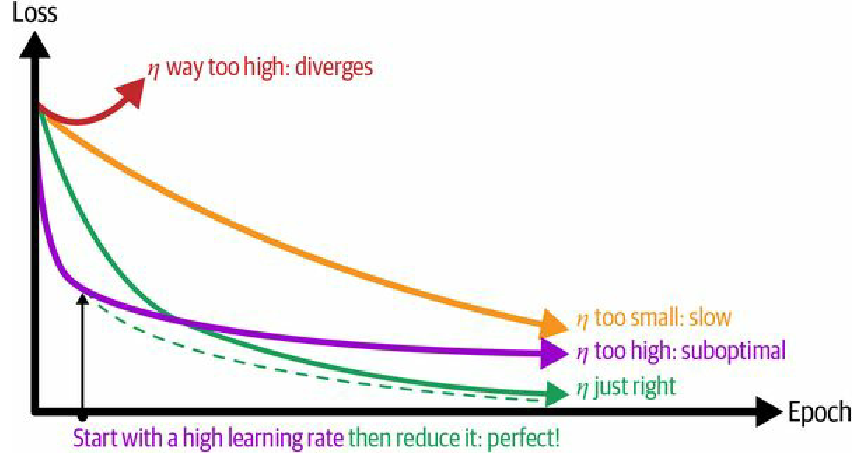
\includegraphics[width=\textwidth]{images/learning rate schedule.png}
        	\tiny{\textit{Nestov momentum\\ Src:Hands-On Machine Learning with Scikit-Learn, Keras, and TensorFlow  Concepts, Tools, and Techniques to Build Intelligent Systems-O'Reilly Media, Inc, Aurélien Géron}}
        \end{column}
	    \begin{column}{0.6\textwidth}
    	    \begin{enumerate}[$\bullet$]
        		\item We have the learning rate high at first so that it gets a relative idea about where the minima lies\pause, and then we lower it to find it with more accuracy\pause
        		\item Scheduling is done on numbers of iterations completed(each iteration is also called an \textit{epoch})\pause
        	\end{enumerate}
    	\end{column}
    \end{columns}
\end{frame}


\begin{frame}{Gradient Descent Statergy- One cycle scheduling}
    \begin{enumerate}[$\bullet$]
		\item The basic idea behind one cycle scheduling is to start with a low learning rate, gradually increase it to a maximum value, and then decrease it again to a low value. This approach helps the network explore a wide range of learning rates, allowing it to quickly converge to a good solution and potentially escape from local minima.
		\item By using a cyclical learning rate schedule, one cycle scheduling aims to strike a balance between exploration and exploitation in the learning process. It enables the network to quickly explore a wide range of learning rates at the beginning and then gradually refine its weights as the learning rate decreases.
    \end{enumerate}
\end{frame}

\begin{frame}{Gradient Descent Strategy- Choosing an activation function}
	\begin{columns}[T]
        \begin{column}{0.5\textwidth}
        	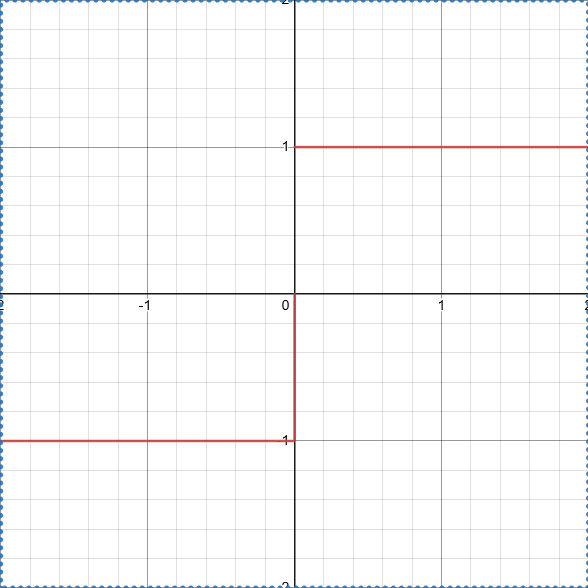
\includegraphics[width=\textwidth]{images/sgn.png}
        	\tiny{\textit{$sgn(x)$}}
        \end{column}
	    \begin{column}{0.5\textwidth}
    	    One of the first activation functions to be considered was $sgn(x)$ mostly because this was the function based on which our neurons operate.
    	\end{column}
    \end{columns}
\end{frame}

\begin{frame}{Gradient Descent Strategy- Choosing an activation function}
	\begin{columns}[T]
        \begin{column}{0.5\textwidth}
        	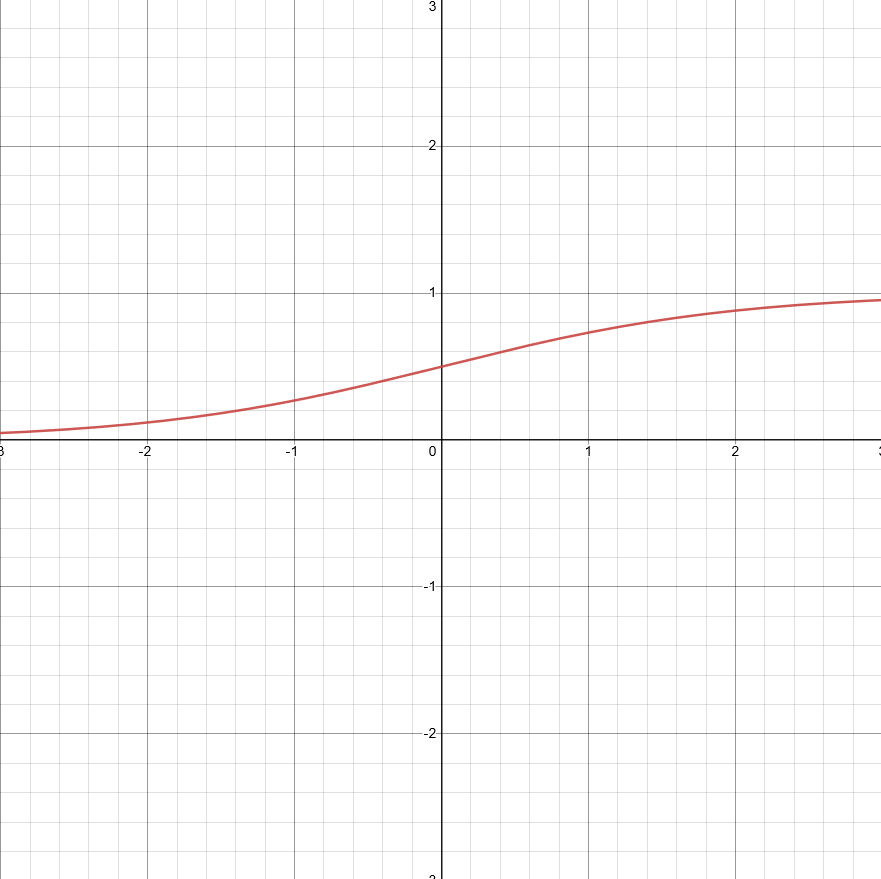
\includegraphics[width=\textwidth]{images/sigmoid.png}
        	\tiny{\textit{$sigmoid$}}
        \end{column}
	    \begin{column}{0.5\textwidth}
    	    But soon better activation functions were found like the \textcolor{red}{sigmoid} function
    	\end{column}
    \end{columns}
\end{frame}

\begin{frame}{Gradient Descent Strategy- Choosing an activation function}
	\begin{columns}[T]
        \begin{column}{0.5\textwidth}
        	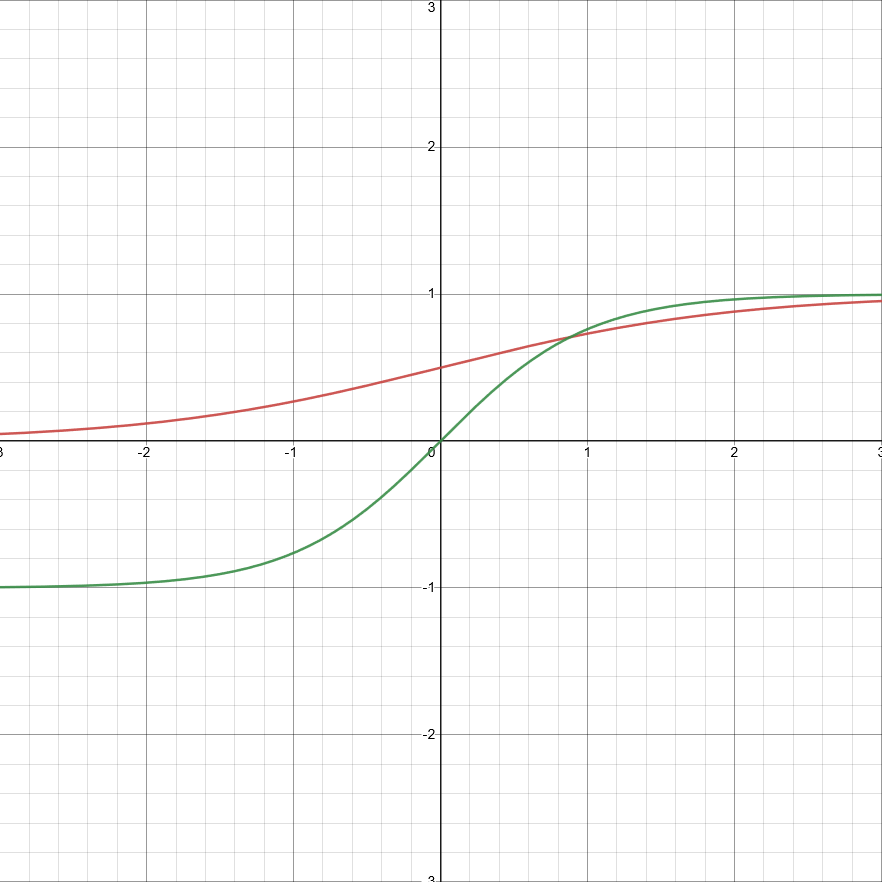
\includegraphics[width=\textwidth]{images/tanh.png}
        	\tiny{\textit{$sigmoid$,$tanh$}}
        \end{column}
	    \begin{column}{0.5\textwidth}
    	    But soon better activation functions were found like the \textcolor{red}{sigmoid} function, \textcolor{green}{tanh} function
    	\end{column}
    \end{columns}
\end{frame}

\begin{frame}{Gradient Descent Strategy- Choosing an activation function}
	\begin{columns}[T]
        \begin{column}{0.5\textwidth}
        	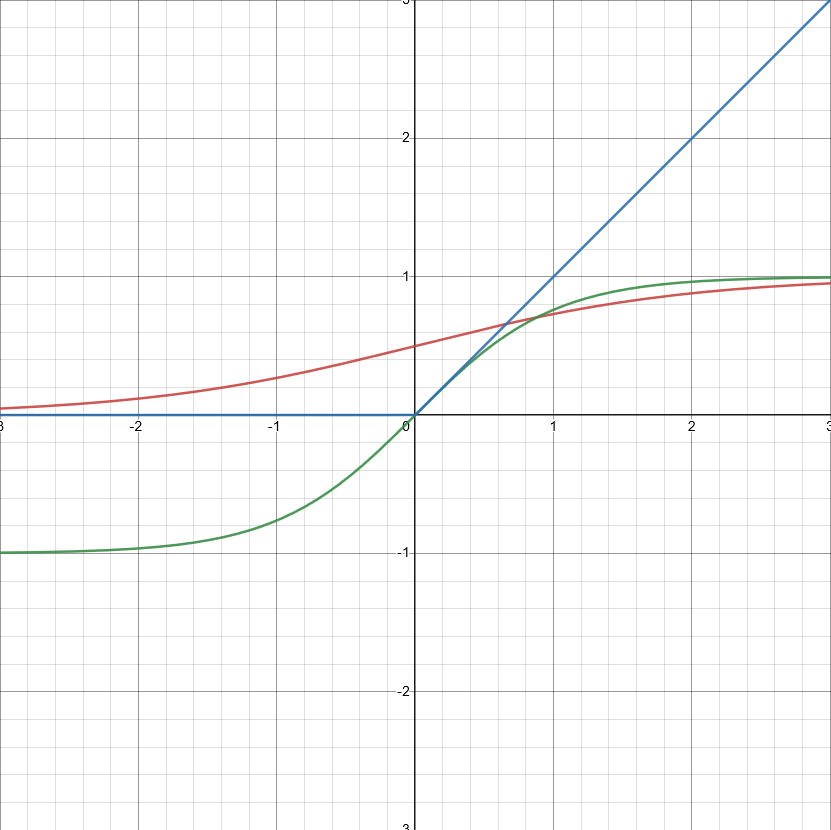
\includegraphics[width=\textwidth]{images/relu.png}
        	\tiny{\textit{$sigmoid$,$tanh$,$relu$}}
        \end{column}
	    \begin{column}{0.5\textwidth}
    	    But soon better activation functions were found like the \textcolor{red}{sigmoid} function, \textcolor{green}{tanh} function and \textcolor{blue}{relu} function.
    	\end{column}
    \end{columns}
\end{frame}

\begin{frame}{Gradient Descent Strategy- Dead Neurons and Vanishing \& Exploding Gradients}
	\begin{columns}[T]
        \begin{column}{0.5\textwidth}
        	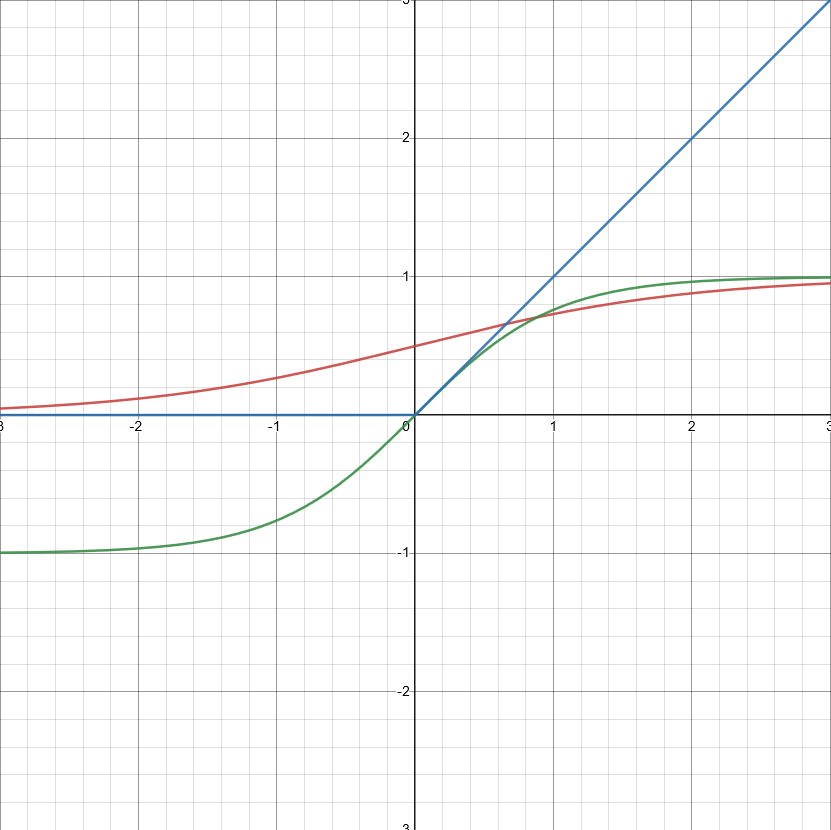
\includegraphics[width=\textwidth]{images/relu.png}
        	\tiny{\textit{$sigmoid$,$tanh$,$relu$}}
        \end{column}
	    \begin{column}{0.5\textwidth}
    	    \begin{enumerate}[$\bullet$]
				\item Most activation function saturated. Therefore, high values meant no gradient "propagated" forward. This leads to neurons which rarely activated and became "dead".\pause 
				\item The effect of derivatives magnifies down the layers. If the order of magnitude is above 1(say $10$) then it explodes(after 10 layers it will become $10^{10}$).
			\end{enumerate}
    	\end{column}
    \end{columns}
\end{frame}

\begin{frame}{Gradient Descent Strategy- Dead Neurons and Vanishing \& Exploding Gradients}
	\begin{columns}[T]
        \begin{column}{0.5\textwidth}
        	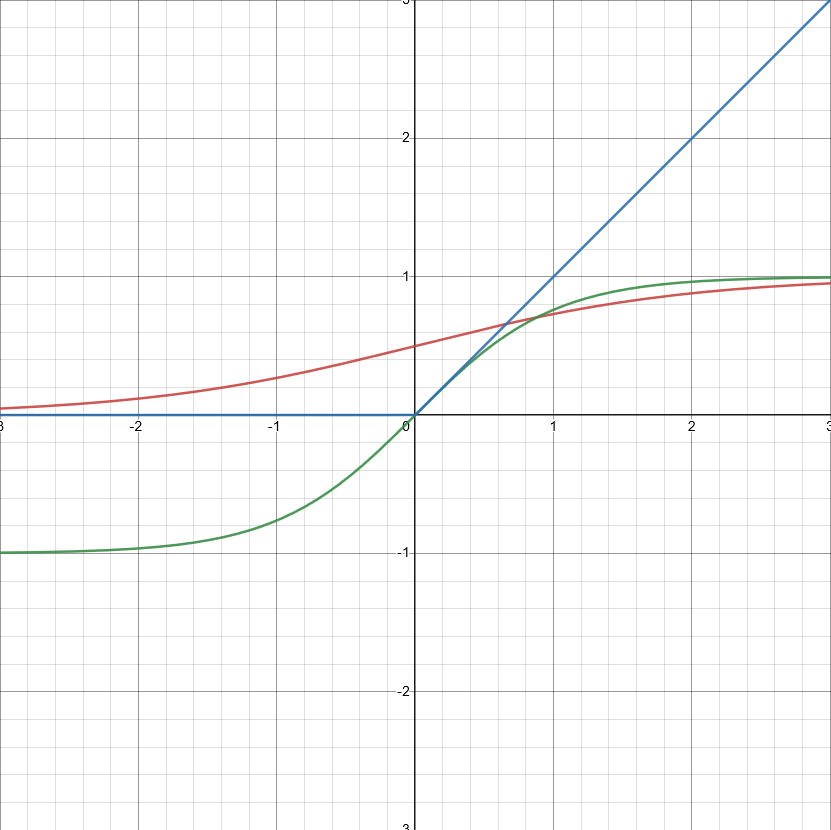
\includegraphics[width=\textwidth]{images/relu.png}
        	\tiny{\textit{$sigmoid$,$tanh$,$relu$}}
        \end{column}
	    \begin{column}{0.5\textwidth}
    	    \begin{enumerate}[$\bullet$]
				\item The effect of derivatives magnifies down the layers. If the order of magnitude is below 1(say $1/10$) then it vanishes(after 10 layers it will become $10^{-10}$)\pause
				\item From a more practical viewpoint, this might lead to overflow if the gradient explodes. If it is vanishing, then there might not be enough precision to handle the values.
			\end{enumerate}
    	\end{column}
    \end{columns}
\end{frame}

\begin{frame}{Gradient Descent Strategy- Better Activation Functions}
	\begin{columns}[T]
        \begin{column}{0.5\textwidth}
        	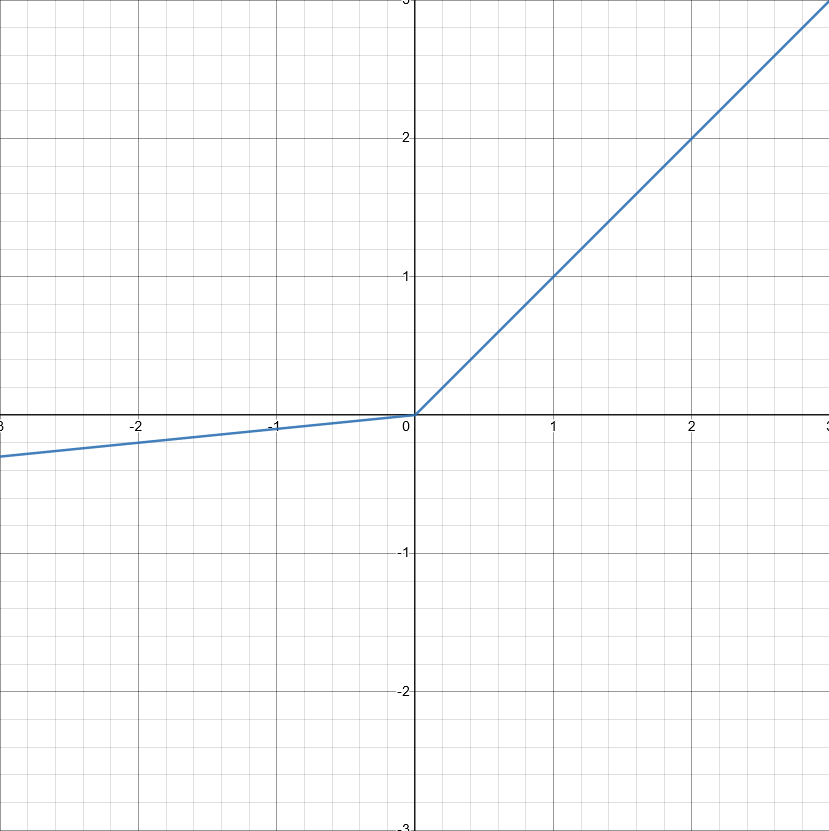
\includegraphics[width=\textwidth]{images/LeakyRelu.png}
        	\tiny{\textit{$leaky$ $ReLu$}}
        \end{column}
	    \begin{column}{0.5\textwidth}
    	    One way to alleviate those problems is to use better activation function which are in a way variants of ReLu. Some examples include 
			\begin{enumerate}[$\bullet$]
				\item \textcolor{blue}{Leaky ReLu $\left(\max(\alpha z,z)\right)$}
			\end{enumerate}
    	\end{column}
    \end{columns}
\end{frame}



\begin{frame}{Gradient Descent Strategy- Better Activation Functions}
	\begin{columns}[T]
        \begin{column}{0.5\textwidth}
        	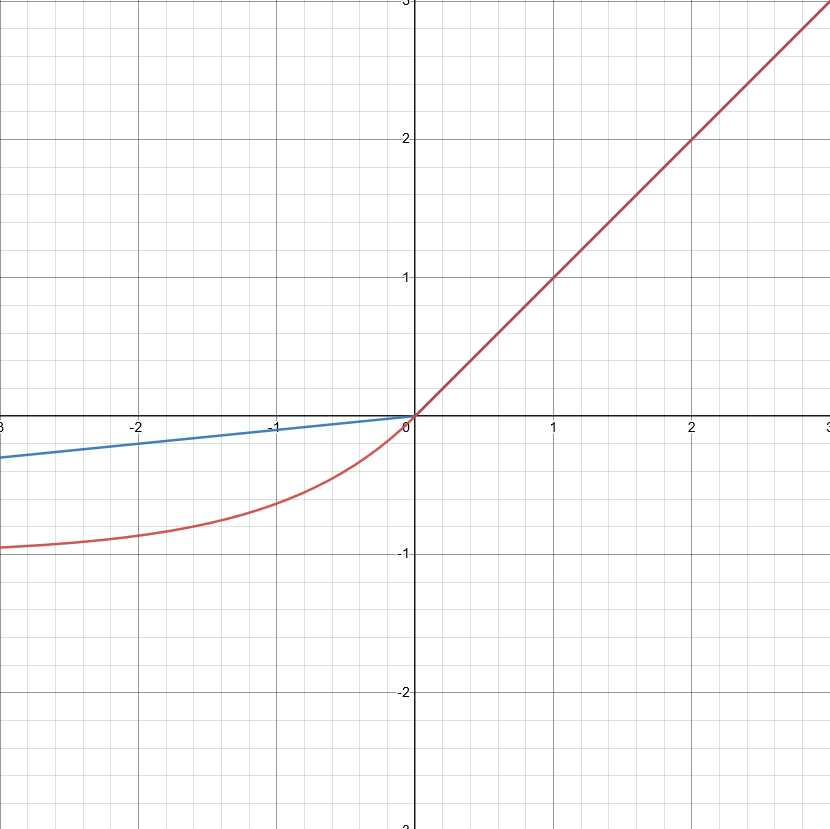
\includegraphics[width=\textwidth]{images/ELU.png}
        	\tiny{\textit{$leaky$ $ReLu$, $ELU$}}
        \end{column}
	    \begin{column}{0.5\textwidth}
    	    One way to alleviate those problems is to use better activation function which are in a way variants of ReLu. Some examples include 
			\begin{enumerate}[$\bullet$]
				\item \textcolor{blue}{Leaky ReLu $\left(\max(\alpha z,z)\right)$}
				\item \textcolor{red}{ELU$\left((\alpha (e^z-1)\text{if $z<0$ else }z)\right)$} 
			\end{enumerate}
    	\end{column}
    \end{columns}
\end{frame}

\begin{frame}{Gradient Descent Strategy- Better Activation Functions}
	\begin{columns}[T]
        \begin{column}{0.5\textwidth}
        	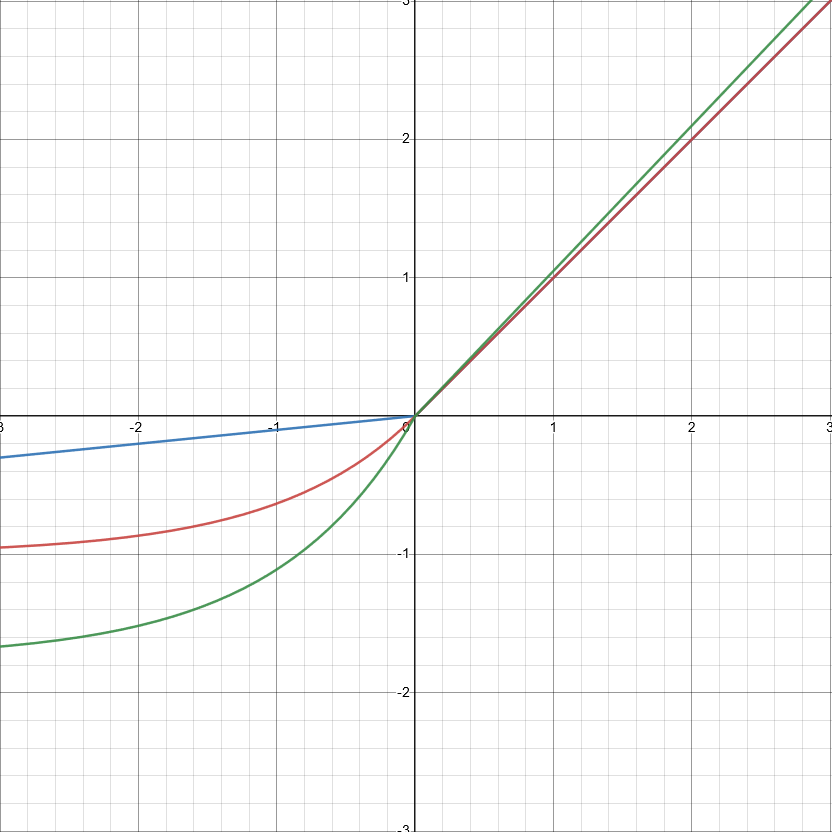
\includegraphics[width=\textwidth]{images/SELU.png}
        	\tiny{\textit{$leaky$ $ReLu$, $ELU$, $SELU$}}
        \end{column}
	    \begin{column}{0.5\textwidth}
    	    One way to alleviate those problems is to use better activation function which are in a way variants of ReLu. Some examples include 
			\begin{enumerate}[$\bullet$]
				\item \textcolor{blue}{Leaky ReLu $\left(\max(\alpha z,z)\right)$}
				\item \textcolor{red}{ELU$\left((\alpha (e^z-1)\text{if $z<0$ else }z)\right)$} 
				\item \textcolor{green}{SELU$\left(1.05ELU_{1.67}\right)$}
			\end{enumerate}
    	\end{column}
    \end{columns}
\end{frame}

\begin{frame}{Gradient Descent Strategy- Better Activation Functions}
	\begin{columns}[T]
        \begin{column}{0.5\textwidth}
        	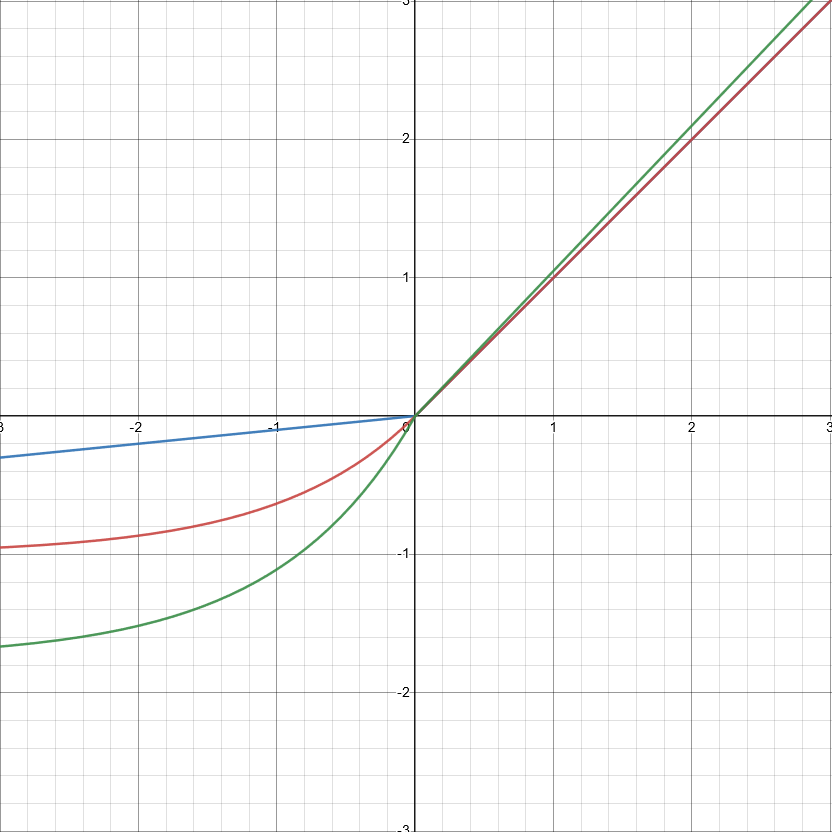
\includegraphics[width=\textwidth]{images/SELU.png}
        	\tiny{\textit{$leaky$ $ReLu$, $ELU$, $SELU$}}
        \end{column}
	    \begin{column}{0.5\textwidth}
    	    One way to alleviate those problems is to use better activation function which are in a way variants of ReLu. Some examples include 
			\begin{enumerate}[$\bullet$]
				\item \textcolor{blue}{Leaky ReLu $\left(\max(\alpha z,z)\right)$}
				\item \textcolor{red}{ELU$\left((\alpha (e^z-1)\text{if $z<0$ else }z)\right)$} 
				\item \textcolor{green}{SELU$\left(1.05ELU_{1.67}\right)$}
			\end{enumerate}
			One can also treat $\alpha$ as a parameter to be learned by back prop. 
    	\end{column}
    \end{columns}
\end{frame}

\begin{frame}{Gradient Descent Strategy- Better Activation Functions}
	\begin{columns}[T]
        \begin{column}{0.5\textwidth}
        	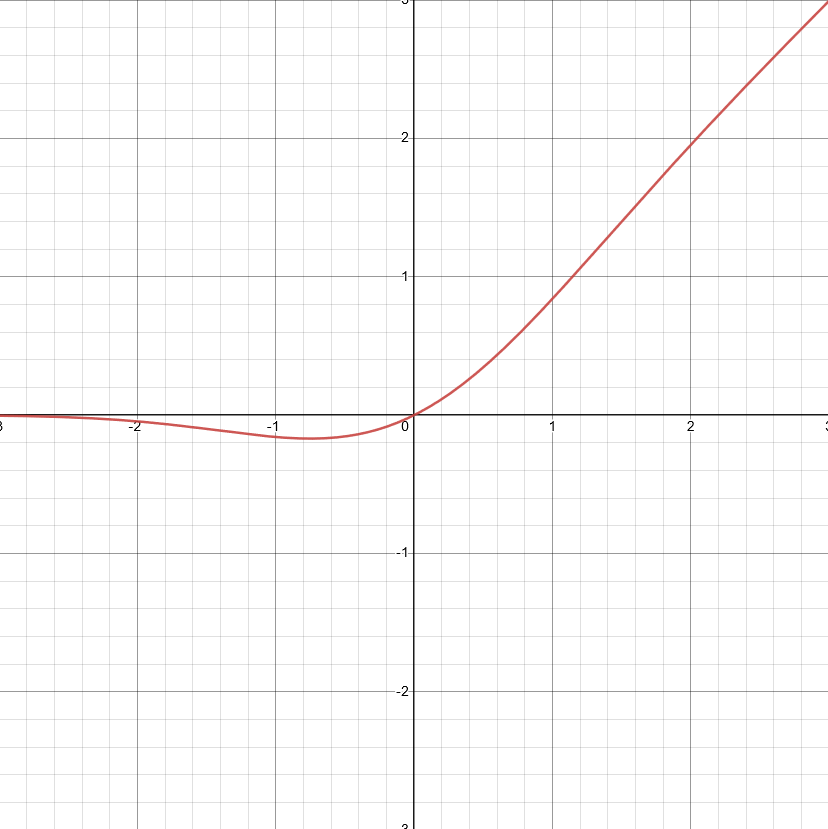
\includegraphics[width=\textwidth]{images/GELU.png}
        \end{column}
	    \begin{column}{0.5\textwidth}
    	    Other activation functions also exists such as 
			\begin{enumerate}[$\bullet$]
				\item \textcolor{blue}{GELU $\left(z\Phi(z)\right)$}where $\Phi$ is the CDF of the standard normal
			\end{enumerate}
    	\end{column}
    \end{columns}
\end{frame}

\begin{frame}{Gradient Descent Strategy- Better Activation Functions}
	\begin{columns}[T]
        \begin{column}{0.5\textwidth}
        	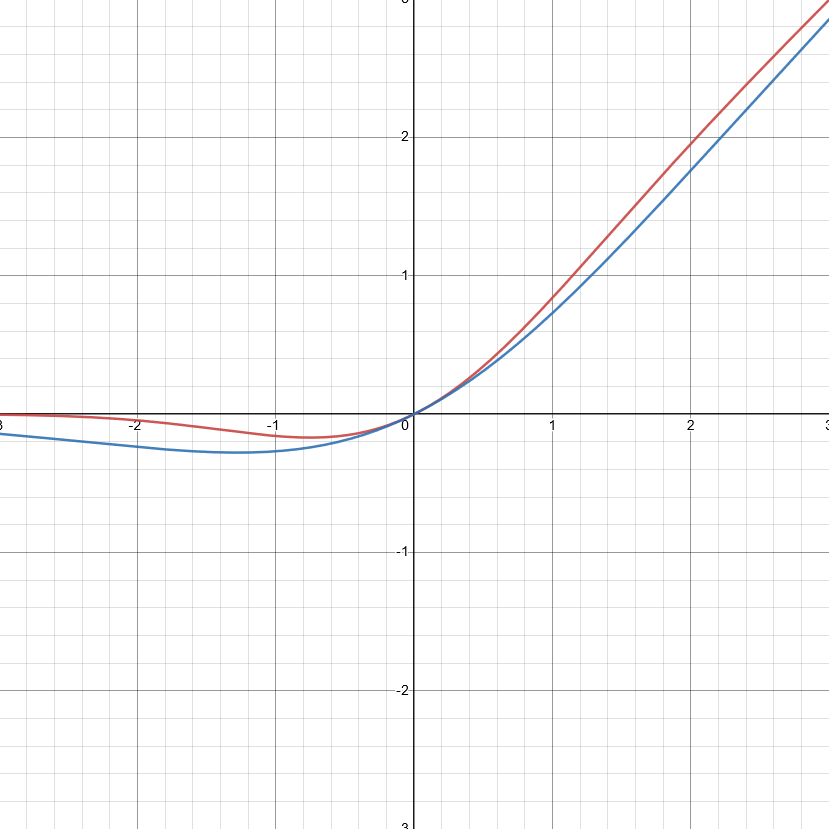
\includegraphics[width=\textwidth]{images/SWISH.png}
        \end{column}
	    \begin{column}{0.5\textwidth}
    	    Other activation functions also exists such as 
			\begin{enumerate}[$\bullet$]
				\item \textcolor{blue}{GELU $\left(z\Phi(z)\right)$}where $\Phi$ is the CDF of the standard normal.
				\item \textcolor{red}{SWISH $\left(z\sigma(z)\right)$}where $\sigma$ is the sigmoid function.
			\end{enumerate}
    	\end{column}
    \end{columns}
\end{frame}

\begin{frame}{Gradient Descent Strategy- Better Activation Functions}
	\begin{columns}[T]
        \begin{column}{0.5\textwidth}
        	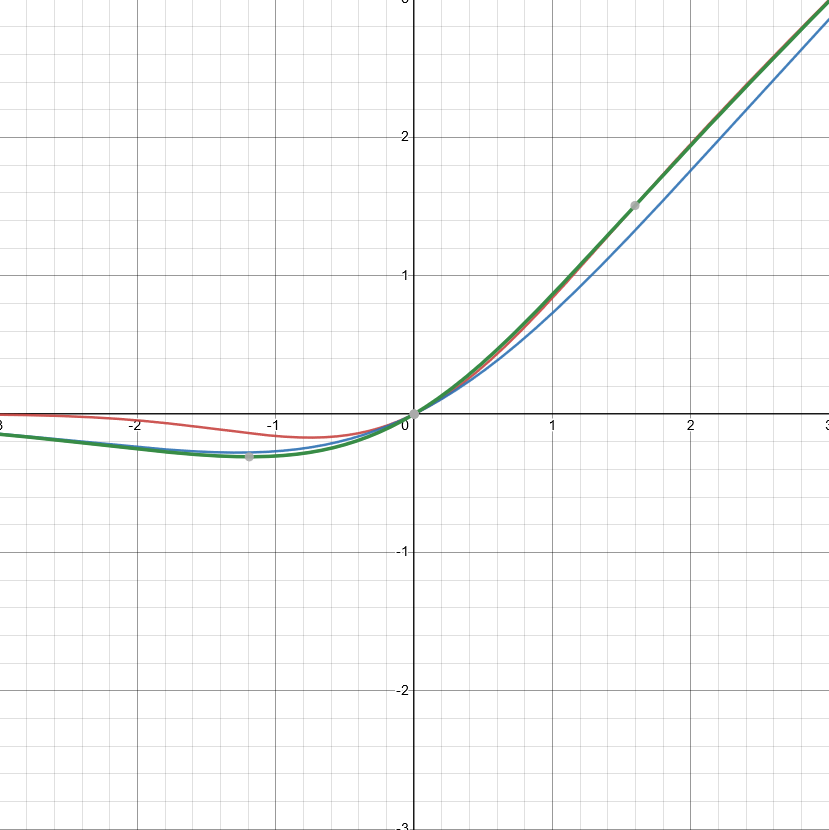
\includegraphics[width=\textwidth]{images/MISH.png}
        \end{column}
	    \begin{column}{0.5\textwidth}
    	    Other activation functions also exists such as 
			\begin{enumerate}[$\bullet$]
				\item \textcolor{blue}{GELU $\left(z\Phi(z)\right)$}where $\Phi$ is the CDF of the standard normal.
				\item \textcolor{red}{SWISH $\left(z\sigma(z)\right)$}where $\sigma$ is the sigmoid function.
				\item \textcolor{green}{MISH $\left(z\tanh(\ln(1+exp(z)))\right)$}where $\sigma$ is the sigmoid function.
			\end{enumerate}
    	\end{column}
    \end{columns}
\end{frame}

\begin{frame}{Gradient Descent Strategy- Weight Initialization}
	\begin{enumerate}[$\bullet$]
		\item Initially weights were initialized by picking from a standard normal distribution.\pause
		\item The difference in the variance of the outgoing nodes and incoming nodes(if there is a difference in number of nodes between layers) cause practical problems in the flow of gradients.\pause
		\item A good compromise is to take average of number of outgoing edges and number of incoming edges and normalize the variance of the normal distribution used by it. This is called Glorot initialization\pause The same principal when used with uniform distribution is called He initialization.
	\end{enumerate}
\end{frame}

\begin{frame}{Gradient Descent Strategy- Gradient Clipping}
	\begin{enumerate}[$\bullet$]
		\item In case one of the components of the gradient is much lager than other we might want to normalize it to control our descent.\pause
		\item One way it to just limit it at some maximum value.\pause
		\item Other methods include normalizing the whole vector with respect to a norm. 
	\end{enumerate}
\end{frame}

\begin{frame}{Aspects of a deep neural network-navigating the loss landscape}
	\begin{enumerate}[$\bullet$]
		\item Generally, as far as decision boundaries are concerned, adding depth gives ore bang for the buck than adding more nodes in a single layer.\pause But depth comes with its own share of problems.\pause
		\item Deeper networks have a harder time converging.\pause
		\item If activation functions are not combined properly then there might be presence of local minimas
	\end{enumerate}
\end{frame}
\begin{frame}{Aspects of a deep neural network-skip connections}
	\begin{columns}[T]
        \begin{column}{0.4\textwidth}
        	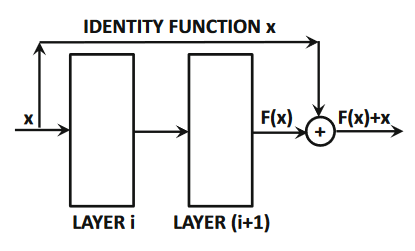
\includegraphics[width=\textwidth]{images/skip.png}
			\tiny{\textit{Skip connections\\ Src:Neural Networks and Deep Learning: A Textbook, Charu C. Aggarwal}}
        \end{column}
	    \begin{column}{0.6\textwidth} 
			\begin{enumerate}[$\bullet$]
				\item We might allow nodes from deeper layers to have direct access to nodes from shallower layers while \textit{skipping} the intermediate layers.\pause
				\item This provides a kind of highway for the deeper layers to access simpler features.\pause
				\item This is especially used in CNNs. A prominent example is the ResNet architecture
			\end{enumerate}
    	\end{column}
    \end{columns}
\end{frame}
\begin{frame}{Aspects of a deep neural network-maxout networks }
	\begin{columns}[T]
        \begin{column}{0.4\textwidth}
        	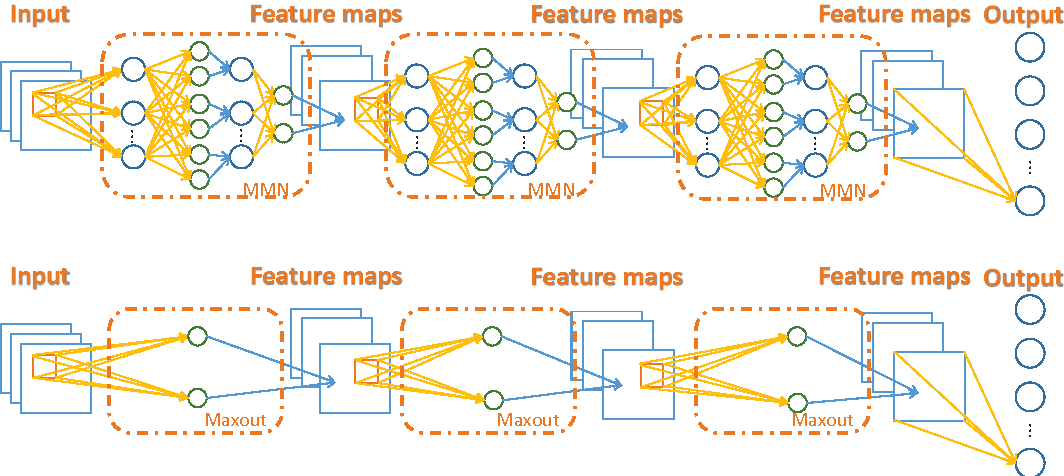
\includegraphics[width=\textwidth]{images/maxout.png}
			\tiny{\textit{Max-out connections\\ Src:Improving deep neural networks with multilayer maxout networks, Weichen Sun, Fei Su, Leiquan Wang}}
        \end{column}
	    \begin{column}{0.6\textwidth} 
			\begin{enumerate}[$\bullet$]
				\item In a certain sense this is type of ensemble method.\pause
				\item Two sets of weights $W_1,W_2$ are trained for each input.
				\item The activation is set to $\sigma\left(\max(W_1\cdot X_{in},W_2\cdot X_{in})+b_0\right)$
			\end{enumerate}
    	\end{column}
    \end{columns}
\end{frame}

\begin{frame}{Aspects of a deep neural network-navigating the loss landscape}
	\begin{enumerate}[$\bullet$]
		\item Generally, as far as decision boundaries are concerned, adding depth gives more bang for the buck than adding more nodes in a single layer.\pause But depth comes with its own share of problems.\pause
		\item Deeper networks have a harder time converging.\pause
		\item If activation functions are not combined properly then there might be presence of local minimas
	\end{enumerate}
\end{frame}

\begin{frame}{Aspects of a deep neural network-Setting hyperparameters}
	\begin{enumerate}[$\bullet$]
		\item Apart from the usual parameters for activation functions, there are other hyperparameters to be set.\pause
		\item Those include stuff like number of layers, number of nodes in a layer, presence and nature of skip connections, presence and nature of max-out layers, choice of activation  functions, choice of learning rates and schedules.\pause
		\item It is not practical to test on the training dataset to prevent overfitting(discussed later) nor is it desired to test on the testing dataset. \pause
		\item In such a scenario using the cross validation set is our best bet.
	\end{enumerate}
\end{frame}

\begin{frame}{Aspects of a deep neural network-Grid Search}
	\begin{enumerate}[$\bullet$]
		\item For setting the hyperparameters we simply choose a possible set of values for each parameter and try everything on the Grid.\pause
		\item We start with coarse grids and then move on to finer ones.
	\end{enumerate}
\end{frame}

\begin{frame}{Practical aspects of a deep neural network-GPU}
	\begin{columns}[T]
        \begin{column}{0.4\textwidth}
        	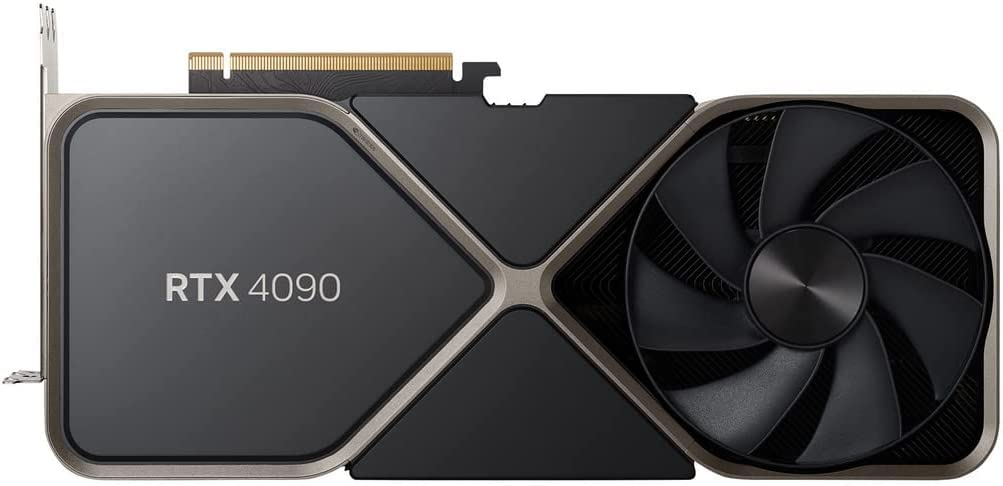
\includegraphics[width=\textwidth]{images/RTX.jpg}
			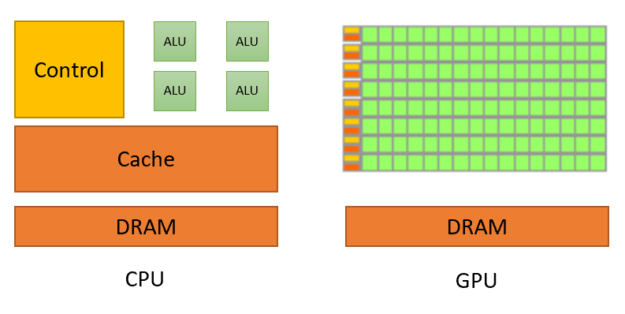
\includegraphics[width=\textwidth]{images/GPUvsCPU.png}
			\tiny{\textit{Comparison of architecture of CPU vs GPU\\ Src:NVIDEA developer's blog}}
        \end{column}
	    \begin{column}{0.6\textwidth} 
			\begin{enumerate}[$\bullet$]
				\item A GPU has more compute units as compared to CPU. It can perform less complicated tasks faster and has the ability to execute the same instruction parallelly. This architecture is often needed in graphics rendering.
				\item A GPU supports the concept of Single Instruction Multiple
				Threads (SIMT) which helps in parallelizing the computation pipeline.
			\end{enumerate}
    	\end{column}
    \end{columns}
\end{frame}

\begin{frame}{Practical aspects of a deep neural network-GPU}
	\begin{columns}[T]
        \begin{column}{0.4\textwidth}
        	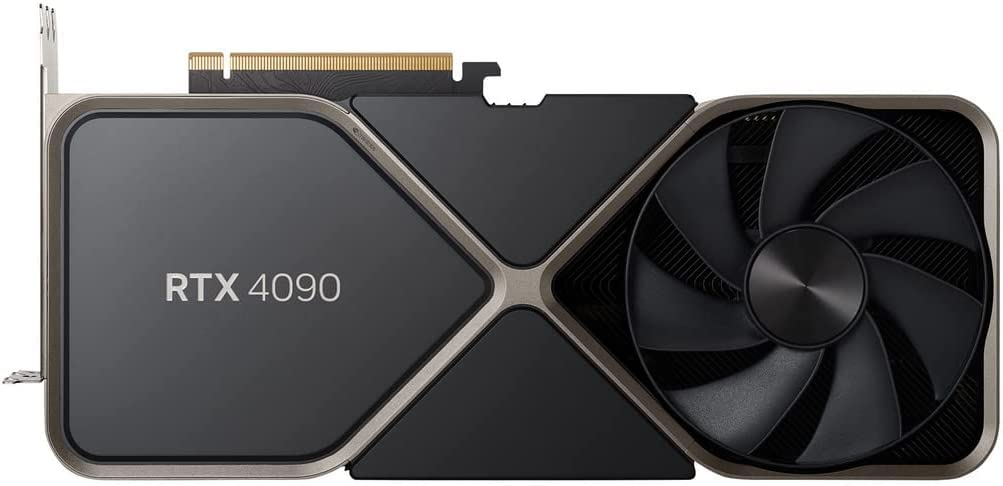
\includegraphics[width=\textwidth]{images/RTX.jpg}
			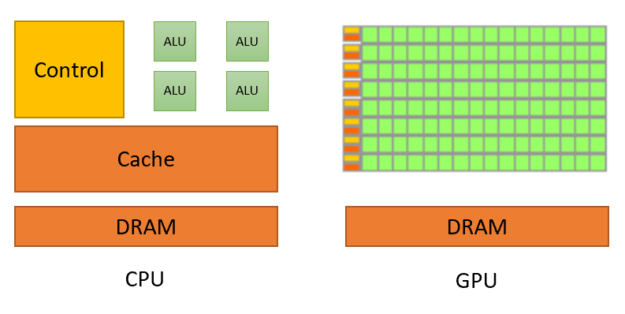
\includegraphics[width=\textwidth]{images/GPUvsCPU.png}
			\tiny{\textit{Comparison of architecture of CPU vs GPU\\ Src:NVIDEA developer's blog}}
        \end{column}
	    \begin{column}{0.6\textwidth} 
			\begin{enumerate}[$\bullet$]
				\item We can use this in back propagation where repeated matrix multiplications are used in the forward phase\pause
				\item Uses can also be found in batch gradient descent(or mini-batch gradient descent) where the same computation is repeated across multiple records.\pause
				\item Often the network is big enough that it doesn't fit in the CPU cache, therefore a CPU has no advantage in terms of bandwidth either. 
			\end{enumerate}
    	\end{column}
    \end{columns}
\end{frame}
\begin{frame}{Practical aspects of a deep neural network- Distributed computation}
	\begin{columns}[T]
        \begin{column}{0.4\textwidth}
        	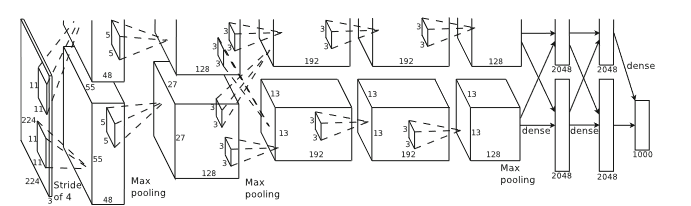
\includegraphics[width=\textwidth]{images/GPU division.png}
			\tiny{\textit{Distributed computation in AlexNet\\ Src:Couldn't trace original source}}
        \end{column}
	    \begin{column}{0.6\textwidth} 
			\begin{enumerate}[$\bullet$]
				\item With GPU partitioning/ Using multiple GPUs, computation can be distributed. \pause
				\item \textbf{Hyperparameter search} We simply run with different hyperparameters on different units to make grid search faster.\pause
				\item  \textbf{Model parallelism} Parts of the model reside in one unit and the rest in others. Examples include Alex-Net which was trained on two GTX 580 GPU. Such models are helpful if and only if the model is large enough to not fit in one GPU: doing this needlessly only increases compute time as data is transferred between different units.
			\end{enumerate}
    	\end{column}
    \end{columns}
\end{frame}

\begin{frame}{Practical aspects of a deep neural network- Distributed computation}
	\begin{columns}[T]
        \begin{column}{0.4\textwidth}
        	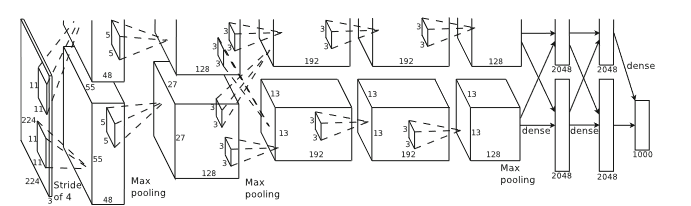
\includegraphics[width=\textwidth]{images/GPU division.png}
			\tiny{\textit{Distributed computation in AlexNet\\ Src:Couldn't trace original source}}
        \end{column}
	    \begin{column}{0.6\textwidth} 
			\begin{enumerate}[$\bullet$]
				\item \textbf{Data parallelism} when the model is small, but there is a large amount of training data, each data can be operated upon in different computational unit and then pooled together.\pause
				\item Hybrid parallelism which combines  parts of all the above models is discussed in One weird trick for parallelizing convolutional neural networks, Alex Krizhevsky
			\end{enumerate}
    	\end{column}
    \end{columns}
\end{frame}

\begin{frame}{Practical aspects of a deep neural network- Pretrained Layers}
	\begin{columns}[T]
        \begin{column}{0.4\textwidth}
        	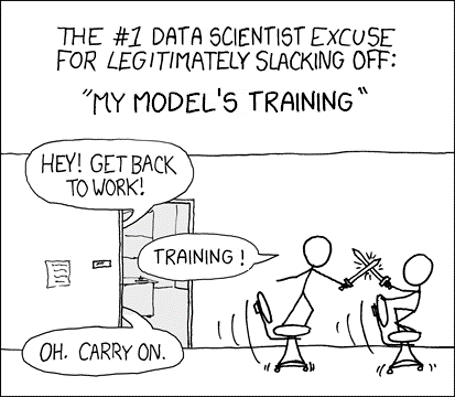
\includegraphics[width=\textwidth]{images/training.png}
			\tiny{\textit{Training\\ Src:XKCD}}
        \end{column}
	    \begin{column}{0.6\textwidth} 
			\begin{enumerate}[$\bullet$]
				\item It takes too long to training neural networks\pause
				\item But one can claim that the low level features remains more or less the same:\pause  We only need to know how to re-combine the high level features and relabel things on the output layer.\pause
				\item We look at some ways to do this. 
			\end{enumerate}
    	\end{column}
    \end{columns}
\end{frame}

\begin{frame}{Practical aspects of a deep neural network- Pretrained Layers}
	\begin{columns}[T]
        \begin{column}{0.4\textwidth}
        	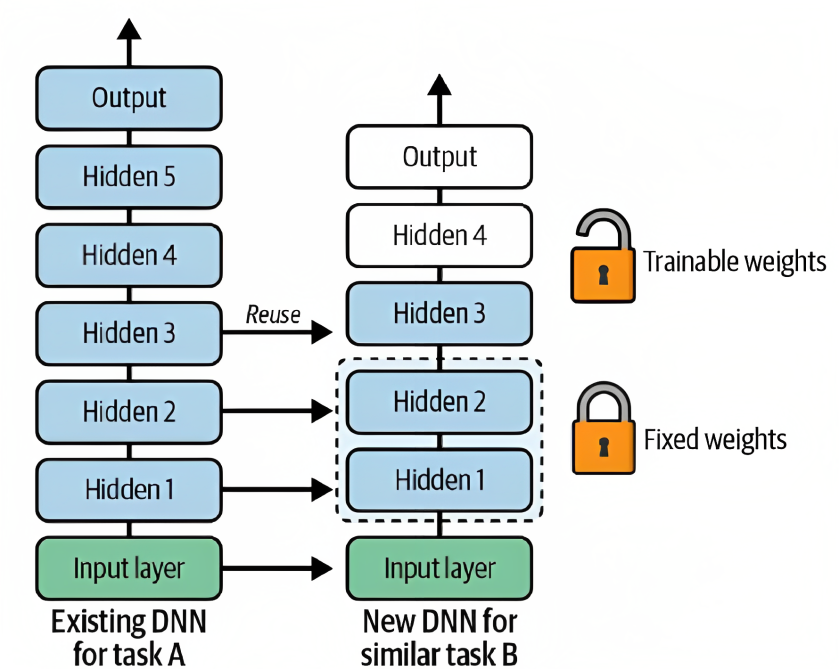
\includegraphics[width=\textwidth]{images/pre-trainedLyers.png}
			\tiny{\textit{Using pre trained layers\\ Src:Hands-On Machine Learning with Scikit-Learn, Keras, and TensorFlow  Concepts, Tools, and Techniques to Build Intelligent Systems-O'Reilly Media, Inc, Aurélien Géron}}
        \end{column}
	    \begin{column}{0.6\textwidth} 
			\begin{enumerate}[$\bullet$]
				\item As mentioned earlier: we argue that low level features can be reused.\pause
				\item There are two ways we might do this:\pause
					\begin{enumerate}[$\bullet$]
						\item Recompute the weights of the higher layers\pause
						\item Remake the higher layers from scratch\pause
					\end{enumerate}
				\item May requires some data strangling. This whole thing is very empirical in nature. Transfer learning works best with deep
				CNNs, which tend to learn feature detectors that are
				much more general (especially in the lower layers)
			\end{enumerate}
    	\end{column}
    \end{columns}
\end{frame}


\begin{frame}{Practical aspects of a deep neural network- Unsupervised Pretraining}
	\begin{columns}[T]
        \begin{column}{0.4\textwidth}
        	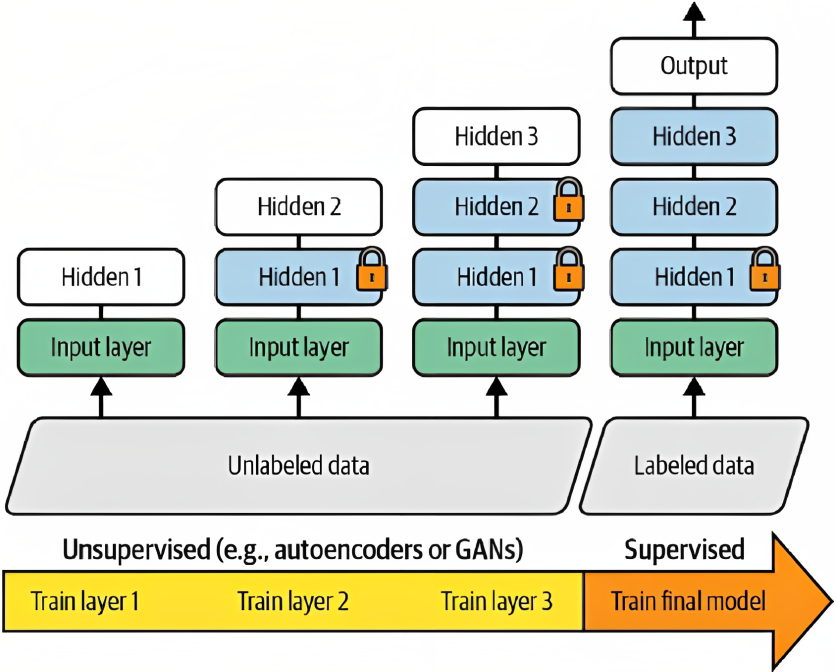
\includegraphics[width=\textwidth]{images/unsupervised pretraining.png}
			\tiny{\textit{Unsupervised pre training\\ Src:Hands-On Machine Learning with Scikit-Learn, Keras, and TensorFlow  Concepts, Tools, and Techniques to Build Intelligent Systems-O'Reilly Media, Inc, Aurélien Géron}}
        \end{column}
	    \begin{column}{0.6\textwidth} 
			\begin{enumerate}[$\bullet$]
				\item In unsupervised training, a model is trained on all data, including the unlabeled data,
				using an unsupervised learning technique, then it is fine-tuned for the final task on just the labeled data
				using a supervised learning technique; the unsupervised part may train one layer at a time as shown
				here, or it may train the full model directly.
				\item Traditionally(upto 2010ish) Random Boltzman Machines(RBMs) were used. Now we use GANs.
			\end{enumerate}
    	\end{column}
    \end{columns}
\end{frame}


\begin{frame}{Practical aspects of a deep neural network- Unsupervised Pretraining}
	\begin{columns}[T]
        \begin{column}{0.4\textwidth}
        	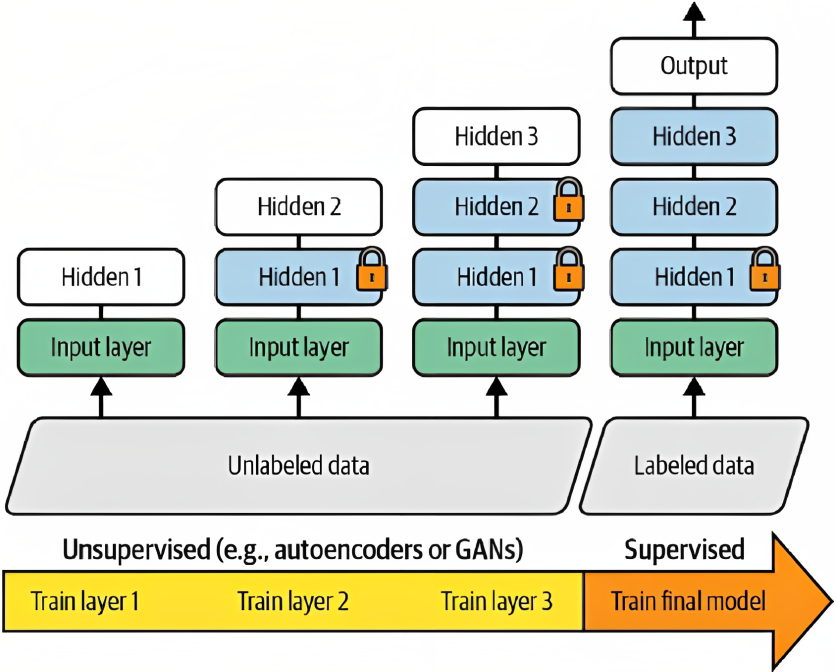
\includegraphics[width=\textwidth]{images/unsupervised pretraining.png}
			\tiny{\textit{Unsupervised pre training\\ Src:Hands-On Machine Learning with Scikit-Learn, Keras, and TensorFlow  Concepts, Tools, and Techniques to Build Intelligent Systems-O'Reilly Media, Inc, Aurélien Géron}}
        \end{column}
	    \begin{column}{0.6\textwidth} 
			\begin{enumerate}[$\bullet$]
				\item Unsupervised pre-training can also be used on auxiliary data.\pause
				\item For example, consider a NLP word prediction case. Even for specialised cases, one doesn't need a specific corpus to predict what comes in \textit{An Apple \textcolor{red}{\_\_} red } 
			\end{enumerate}
    	\end{column}
    \end{columns}
\end{frame}


usebackgroundtemplate{%             declare it
\tikz[overlay,remember picture] \node[opacity=1, at=(current page.center)] {
   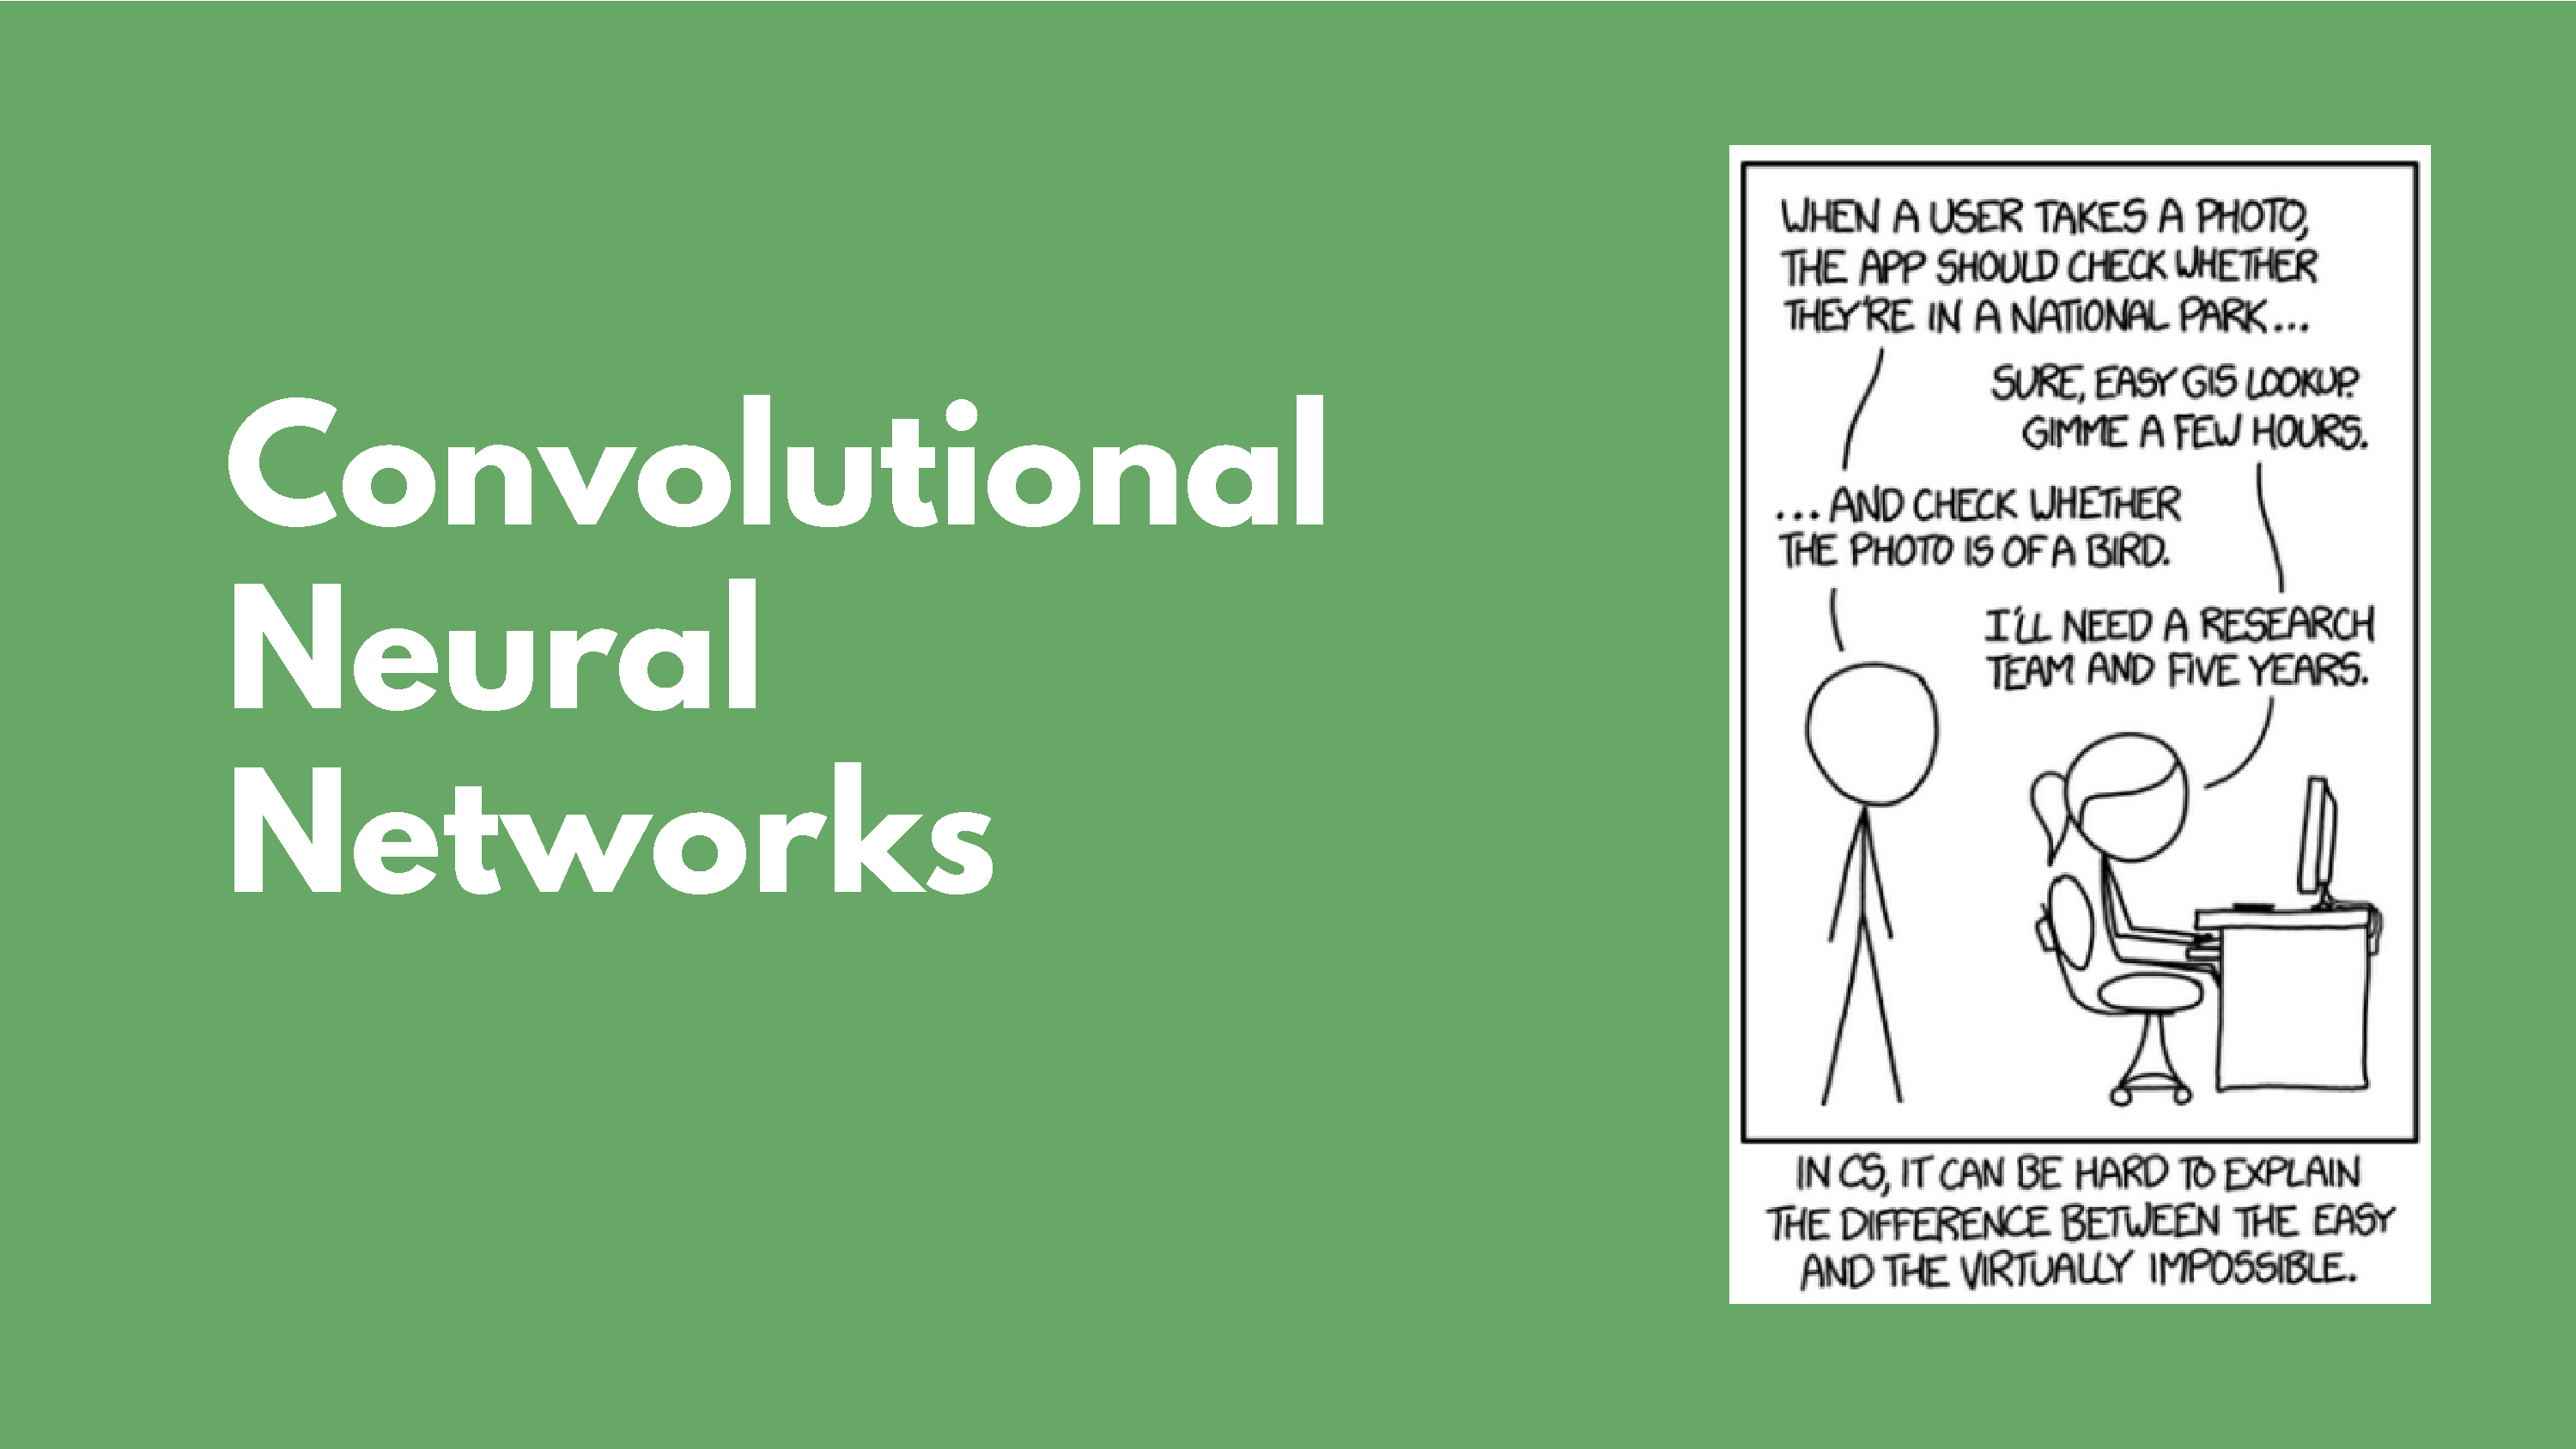
\includegraphics[height=\paperheight,width=\paperwidth]{images/cnn.pdf}};
}
\begin{frame}
\end{frame}

\usebackgroundtemplate{ }

\begin{frame}{Why CNN?}
	\begin{columns}[T]
        \begin{column}{0.4\textwidth}
			\begin{center}
				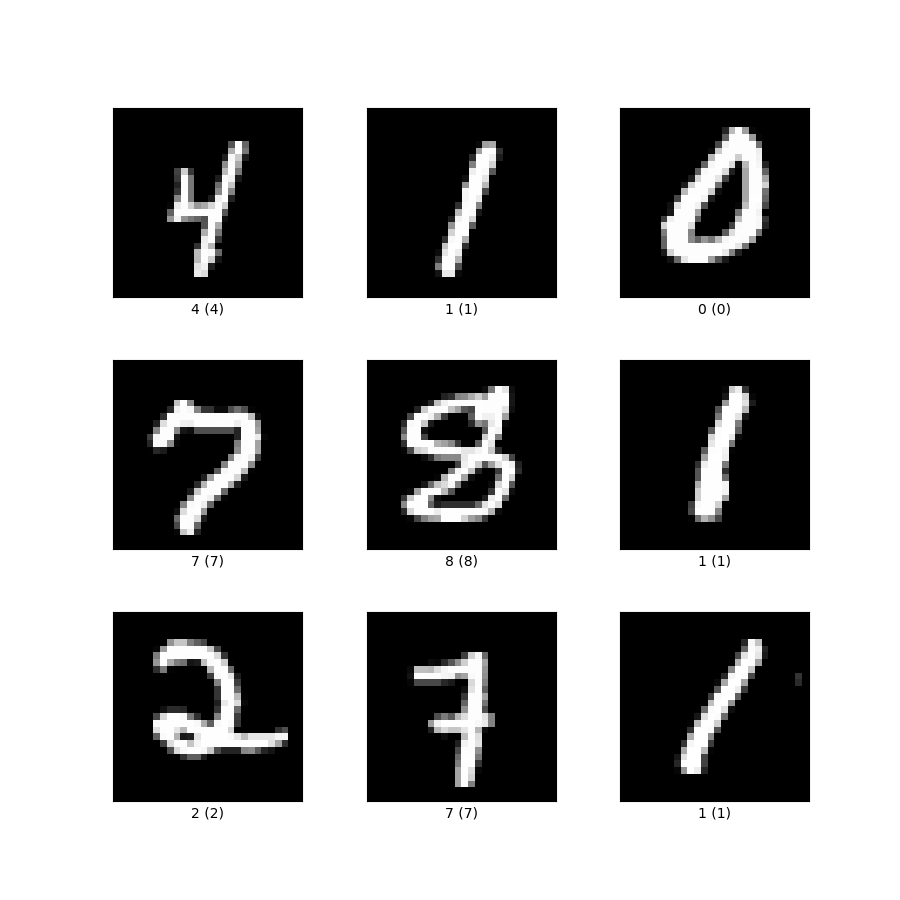
\includegraphics[width=0.5\textwidth]{images/mnist.png}\\
				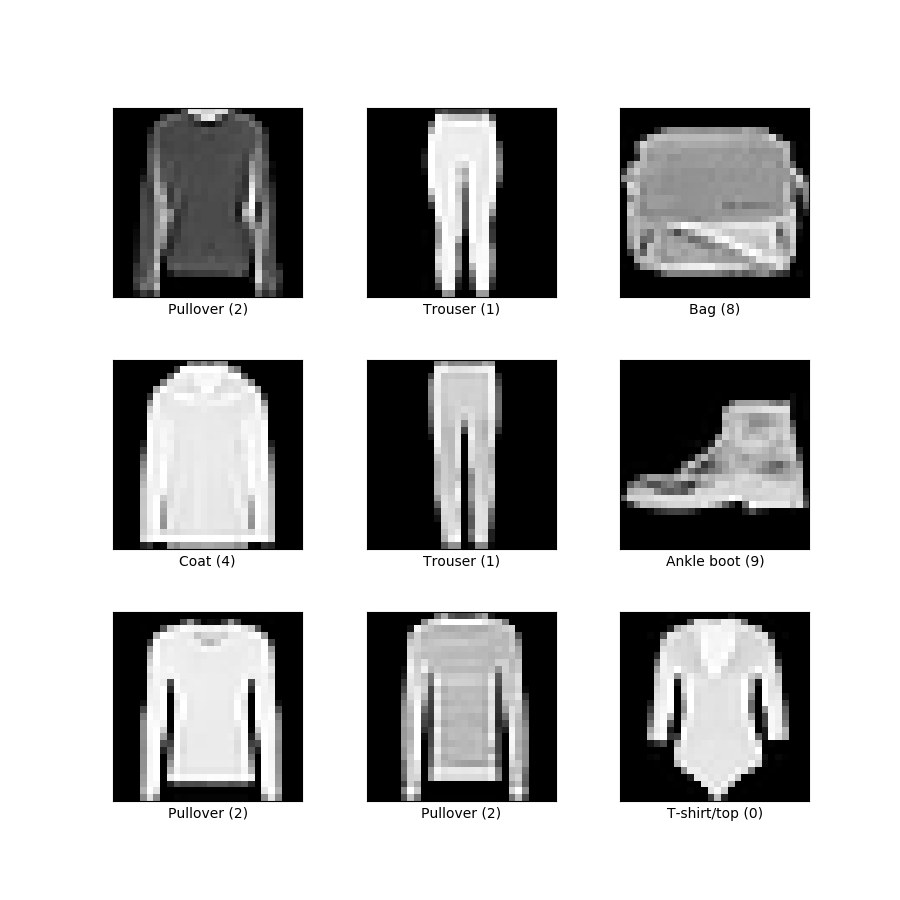
\includegraphics[width=0.5\textwidth]{images/mnist_f.png}\\
			\end{center}
			\tiny{\textit{Samples from the MNIST handwriting and fashion dataset\\ Src: www.TensorFlow.org}}
        \end{column}
	    \begin{column}{0.6\textwidth} 
			For images the spatial arrangement of the pixels matter. Therefore, it is unintuitive for dense layers to perform well as all the spatial information is lost.\\\pause
			We again take inspiration from biology. Hubel and Wiesel's work showed certain neurons were triggered when particular patterns were seen by the eye. We take a similar approach and use activation functions which search for specific patterns.
    	\end{column}
    \end{columns}
\end{frame}

\begin{frame}{Convolutional Filters}
	\begin{columns}[T]
        \begin{column}{0.5\textwidth}
        	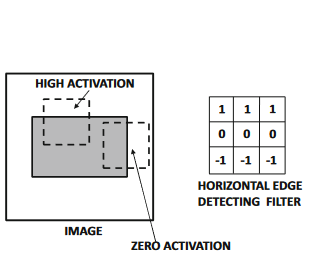
\includegraphics[width=\textwidth]{images/CNN_filter.png}
			\tiny{\textit{CNN filter to detect horizontal edges\\Src:Neural Networks and Deep Learning: A Textbook, Charu C. Aggarwal }}
        \end{column}
	    \begin{column}{0.5\textwidth} 
			We "look for" low level features by taking a matrix which gives a high value on element-wise product and then summing when it detects a feature and preferably 0 or some  other low-value otherwise. We don't create the filters, we let the machine learn them. The output of an image after a particular filter is applied is the feature map corresponding to the feature the filter is trying to capture.
    	\end{column}
    \end{columns}
\end{frame}

\begin{frame}{Convolutional Filters}
	\begin{columns}[T]
        \begin{column}{0.5\textwidth}
        	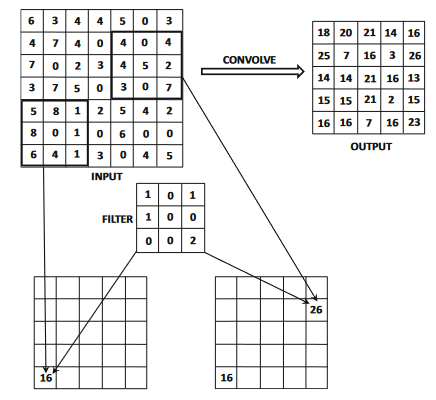
\includegraphics[width=\textwidth]{images/CNN_filter_ex.png}
			\tiny{\textit{Example of a CNN filter\\Src:Neural Networks and Deep Learning: A Textbook, Charu C. Aggarwal }}
        \end{column}
		\begin{column}{0.5\textwidth}
	    An example is show on the left. If we convolve with some "stride" or space between consecutive placement of filters, we are also looking to reducing the dimension of the image: essentially a reduction in number of parameters to be considered.
		\end{column} 
    \end{columns}
\end{frame}

\begin{frame}{Convolutional Filters}
	\begin{columns}[T]
        \begin{column}{0.5\textwidth}
        	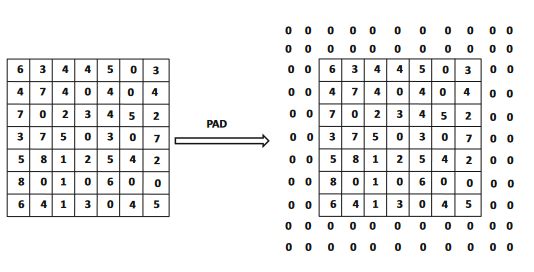
\includegraphics[width=\textwidth]{images/CNN_filter_pad.png}
			\tiny{\textit{Example of a CNN filter with padding\\Src:Neural Networks and Deep Learning: A Textbook, Charu C. Aggarwal }}
        \end{column}
		\begin{column}{0.5\textwidth}
			We might make it so that we simply don't go far enough towards the edges that the filter gets stuck. Another method is to "pad" the edges with 0 
		\end{column} 
    \end{columns}
\end{frame}

\begin{frame}{Pooling Filters}
	\begin{columns}[T]
        \begin{column}{0.5\textwidth}
        	\includegraphics[width=\textwidth]{images/CNN_pool.png}
			\tiny{\textit{Example of a CNN filter\\Src:Neural Networks and Deep Learning: A Textbook, Charu C. Aggarwal }}
        \end{column}
		\begin{column}{0.5\textwidth}
	    We consider another type of filter called a pooling filter. This essentially captures the "essence" of the part of the image where the filter is placed making by only taking the max value while making it indifferent to small changes in the picture. The goal is to decrease the size by subsampling while retaining the useful features
		
		\end{column} 
    \end{columns}
\end{frame}

\begin{frame}{Pooling Filters-invariance}
	\begin{columns}[T]
		\begin{column}{0.5\textwidth}
        	\includegraphics[width=\textwidth]{images/inv ex.png} 
        \end{column}
        \begin{column}{0.5\textwidth}
        	\includegraphics[width=\textwidth]{images/pooling_inv.png}
        \end{column}
    \end{columns}
	\tiny{\textit{Invariance due to pooling\\ Src:Hands-On Machine Learning with Scikit-Learn, Keras, and TensorFlow  Concepts, Tools, and Techniques to Build Intelligent Systems-O'Reilly Media, Inc, Aurélien Géron}}
\end{frame}


\begin{frame}{Data augmentation}
	\begin{columns}[T]
        \begin{column}{0.4\textwidth}
        	\includegraphics[width=\textwidth]{images/Data Aug.png}
			\tiny{\textit{Example of a data augmentation\\ Src:Hands-On Machine Learning with Scikit-Learn, Keras, and TensorFlow  Concepts, Tools, and Techniques to Build Intelligent Systems-O'Reilly Media, Inc, Aurélien Géron}}
        \end{column}
		\begin{column}{0.6\textwidth}
			\begin{enumerate}[$\bullet$]
				\item Data augmentation artificially increases the size of the training set by
				generating many realistic variants of each training instance. This reduces
				overfitting, making this a regularization technique.\pause
				\item Simply adding white noise will not help; the
				modifications should be learnable. The generated
				instances should be as realistic as possible: ideally, given an image from
				the augmented training set, a human should not be able to tell whether it
				was augmented or not.
			\end{enumerate}
		\end{column} 
    \end{columns}
\end{frame}
\begin{frame}{Data augmentation}
	\begin{columns}[T]
        \begin{column}{0.4\textwidth}
        	\includegraphics[width=\textwidth]{images/Data Aug.png}
			\tiny{\textit{Example of a data augmentation\\ Src:Hands-On Machine Learning with Scikit-Learn, Keras, and TensorFlow  Concepts, Tools, and Techniques to Build Intelligent Systems-O'Reilly Media, Inc, Aurélien Géron}}
        \end{column}
		\begin{column}{0.6\textwidth}
			\begin{enumerate}[$\bullet$]
				\item For example, you can slightly shift, rotate, and resize every picture in the
				training set by various amounts and add the resulting pictures to the
				training set. This forces the model to be more tolerant to
				variations in the position, orientation, and size of the objects in the
				pictures. \pause
				\item To produce a model that's more tolerant of different lighting
				conditions, you can similarly generate many images with various
				contrasts. 
			\end{enumerate}
		\end{column} 
    \end{columns}
\end{frame}
\begin{frame}{Inception Module}
	\begin{columns}[T]
        \begin{column}{0.4\textwidth}
        	\includegraphics[width=\textwidth]{images/Inception module without bottlenecks.png}
			\tiny{\textit{Schematic of an Inception Module\\ Src:Hands-On Machine Learning with Scikit-Learn, Keras, and TensorFlow  Concepts, Tools, and Techniques to Build Intelligent Systems-O'Reilly Media, Inc, Aurélien Géron }}
        \end{column}
		\begin{column}{0.6\textwidth}
			\begin{enumerate}[$\bullet$]
				\item Instead of deciding what size of filter, or which filter to use, we kind of do all of them together.\pause
				\item The 1$\times$1 filters are kept to:
					\begin{enumerate}[$\bullet$]
						\item They can capture patterns
						along the depth dimension\pause
						\item They are configured to output fewer feature maps than their inputs, so
						they serve as bottleneck layers, meaning they reduce dimensionality.\pause
					\end{enumerate}
				\item The whole thing can be though of applying a single filter but on steroids.
			\end{enumerate}
		\end{column} 
    \end{columns}
\end{frame}
\begin{frame}{Inception Module}
	\includegraphics[width=\textwidth]{images/Inception module with bottlenecks.png}
	\tiny{\textit{Schematic of an Inception Module with and without bottlenecks\\ Src:Neural Networks and Deep Learning: A Textbook, Charu C. Aggarwal }}
\end{frame}
\begin{frame}{Res-Net Skip connections}
	\begin{enumerate}[$\bullet$]
		\item CNNs also use skip connections
		\item The main idea is only essential high level features propagate forward.
		\item The higher layers may learn faster than the shallower layers due to presence of low level feature highways.
	\end{enumerate}
\end{frame}

\begin{frame}{Squeeze and excite architecture}
	\begin{columns}[T]
        \begin{column}{0.4\textwidth}
        	\includegraphics[width=\textwidth]{images/S&E.png}
			\tiny{\textit{Squueze and excite architecture\\ Src:Hands-On Machine Learning with Scikit-Learn, Keras, and TensorFlow  Concepts, Tools, and Techniques to Build Intelligent Systems-O'Reilly Media, Inc, Aurélien Géron }}
        \end{column}
		\begin{column}{0.6\textwidth}
			\begin{enumerate}[$\bullet$]
				\item The idea stems from the fact that not all features are equally important.\pause
				\item To recognize the essential feature we train a shallow neural network and scale the feature map  with respect to the outputs. \pause
				\item This is essentially a cross feature map transformation and less of a within feature transformation.
			\end{enumerate}
		\end{column} 
    \end{columns}
\end{frame}
\begin{frame}{Squeeze and excite architecture}
	\includegraphics[width=\textwidth]{images/SEoverview.png}
	\tiny{\textit{Squeeze and Excititation overview\\ Src:Neural Networks and Deep Learning: A Textbook, Charu C. Aggarwal }}
\end{frame}
\begin{frame}{Squeeze and excite architecture}
	\begin{center}
		\includegraphics[width=0.69\textwidth]{images/SE implementations.png}%nice~
	\end{center}
	\tiny{\textit{Squeeze and Excite Implementation\\ Src:Hands-On Machine Learning with Scikit-Learn, Keras, and TensorFlow  Concepts, Tools, and Techniques to Build Intelligent Systems-O'Reilly Media, Inc, Aurélien Géron  }}
\end{frame}

\begin{frame}{Object localization}
	\begin{columns}[T]
        \begin{column}{0.4\textwidth}
        	\includegraphics[width=\textwidth]{images/loca.png}
			\tiny{\textit{Object localization\\Src:Video C4W3L02 by DeepLearningAI, Andrew Ng}}
        \end{column}
		\begin{column}{0.6\textwidth}
			\begin{enumerate}[$\bullet$]
				\item We would like to detect the location (or absence) of an object in an image.\pause
				\item This is a two-part process: We need to recognize that there is an object centered in the bounding box, and then we identify what object it is. \pause
				\item This can be done together by taking them to be output of a single Neural Network. For example Output 1 to 10 gives class probability, output 11 gives objectness probability, output 12-15 gives opposite corners of the bounding box.
			\end{enumerate}
		\end{column} 
    \end{columns}
\end{frame}
\begin{frame}{Object localization}
	\begin{columns}[T]
        \begin{column}{0.4\textwidth}
        	\includegraphics[width=\textwidth]{images/landmark detection.png}
			\tiny{\textit{Object localization\\ Src:Video C4W3L02 by DeepLearningAI, Andrew Ng}}
        \end{column}
		\begin{column}{0.6\textwidth}
			\begin{enumerate}[$\bullet$]
				\item It might lead to detection of the same object multiple times. To prevent this we might discard overlapping boxes whose object detection confidence is low.\pause
				\item Instead of bounding boxes we might also try to detect landmarks such as corners of eyes, border of face, lips etc. They are an integral part of emotion recognition from images and augmented reality
			\end{enumerate}
		\end{column} 
    \end{columns}
\end{frame}

\begin{frame}{Object detection by sliding window}
	\begin{columns}[T]
        \begin{column}{0.4\textwidth}
        	\includegraphics[width=\textwidth]{images/object detecton sliding CNN.png}
			\tiny{\textit{Object detection by sliding window\\ Src:Hands-On Machine Learning with Scikit-Learn, Keras, and TensorFlow  Concepts, Tools, and Techniques to Build Intelligent Systems-O'Reilly Media, Inc, Aurélien Géron }}
        \end{column}
		\begin{column}{0.6\textwidth}
			\begin{enumerate}[$\bullet$]
				\item For detecting multiple object in a single image, one might use a sliding window of boxes and run object detection in each of them.
				\item It might lead to detection of the same object multiple times. To prevent this we might discard overlapping boxes whose object detection confidence is low.\pause
				\item This is computationally expensive
			\end{enumerate}
		\end{column} 
    \end{columns}
\end{frame}

\begin{frame}{Fully Convolutional Networks(FCN)}
	\begin{columns}[T]
        \begin{column}{0.4\textwidth}
        	\includegraphics[width=\textwidth]{images/FCN.png}
			\tiny{\textit{FCN\\ Src:Hands-On Machine Learning with Scikit-Learn, Keras, and TensorFlow  Concepts, Tools, and Techniques to Build Intelligent Systems-O'Reilly Media, Inc, Aurélien Géron }}
        \end{column}
		\begin{column}{0.6\textwidth}
			\begin{enumerate}[$\bullet$]
				\item Consider a CNN which does single class prediction on a 224$\times$224 image and outputs a class prediction probability output, an objectness probability output and a bounding box.\pause
				\item We might consider this particular network as a filter in itself and run it on larger images.\pause
				\item We are therefore essentially removing dense layers and replacing it with an convolutional layer.
			\end{enumerate}
		\end{column} 
    \end{columns}
\end{frame}

\begin{frame}{YOLO: You only look once}
	\begin{columns}[T]
        \begin{column}{0.4\textwidth}
        	\includegraphics[width=\textwidth]{images/YOLO.png}
			\tiny{\textit{YOLO\\Src:Video C4W3L09 by DeepLearningAI, Andrew Ng }}
        \end{column}
		\begin{column}{0.6\textwidth}
			\begin{enumerate}[$\bullet$]
				\item For each class, the machine learns the approximate shape of the object bounding box. This is an anchor\pause
				\item The image is divided in a grid and for each grid object localization is done. For object of class $i$, the bounding box is chosen such that it is most similar in shape to anchor of class $i$.
			\end{enumerate}
		\end{column} 
    \end{columns}
\end{frame}

usebackgroundtemplate{%             declare it
\tikz[overlay,remember picture] \node[opacity=1, at=(current page.center)] {
   \includegraphics[height=\paperheight,width=\paperwidth]{images/RNN.pdf}};
}
\begin{frame}
\end{frame}

\usebackgroundtemplate{ }

\begin{frame}{Why RNN?}
	\begin{columns}[T]
        \begin{column}{0.7\textwidth}
			\includegraphics[width=\textwidth]{images/why RNN.png}
			\tiny{\textit{Why RNN is needed\\Src:Neural Networks and Deep Learning: A Textbook, Charu C. Aggarwal }}
        \end{column}
	    \begin{column}{0.3\textwidth} 
			RNN is used on data with a temporal sequence. For sequences like text, what comes after another words plays an important role. We also need to factor in the fact that there is 1 dimension to consider and the sequence length may vary. 
    	\end{column}
    \end{columns}
\end{frame}

\begin{frame}{RNN variants}
	\begin{center}
		\includegraphics[width=0.8\textwidth]{images/RNN variant.png}
	\end{center}
	\tiny{\textit{RNN variants with respect to different inputs and outputs\\Src:Neural Networks and Deep Learning: A Textbook, Charu C. Aggarwal }}
\end{frame}
\begin{frame}{RNN Structure and Trainig}
	\begin{columns}[T]
        \begin{column}{0.4\textwidth}
        	\includegraphics[width=\textwidth]{images/RNN struct.png}
			\tiny{\textit{Structure of an RNN\\Src:Neural Networks and Deep Learning: A Textbook, Charu C. Aggarwal  }}
        \end{column}
		\begin{column}{0.6\textwidth}
			\begin{enumerate}[$\bullet$]
				\item A sequence starts with a $start$ and $end$ tokem\pause
				\item We assume $W_{xh},W_{hh},W_{hy}$ remains constant.\pause
				\item We use back propagation through time to calculate all parameters.\pause Note, since the temporal sequence matters, we can no longer use stochastic/mini batch gradient descent methods. This is a reason why training RNN is difficult.
			\end{enumerate}
		\end{column} 
    \end{columns}
\end{frame}

\begin{frame}{Bidirectional RNN}
	\begin{columns}[T]
        \begin{column}{0.4\textwidth}
        	\includegraphics[width=\textwidth]{images/BiRNN.png}
			\tiny{\textit{Structure of an Bidirectional RNN\\Src:Neural Networks and Deep Learning: A Textbook, Charu C. Aggarwal  }}
        \end{column}
		\begin{column}{0.6\textwidth}
			\begin{enumerate}[$\bullet$]
				\item Note that going in one direction is not always accurate: for languages text which is going to appear later might influence text which is predicted now. 
				\item A toy example might be \textit{"She has  a \textcolor{red}{\_\_} \textcolor{blue}{apple}"} vs \textit{"She has  a \textcolor{red}{\_\_} \textcolor{blue}{banana}"} 
				\item Therefore, we might go bi directionally during training to make the network more robust.
			\end{enumerate}
		\end{column} 
    \end{columns}
\end{frame}

\begin{frame}{The problem with RNN}
	\begin{columns}[T]
        \begin{column}{0.4\textwidth}
        	\includegraphics[width=\textwidth]{images/RNN struct.png}
			\tiny{\textit{Structure of an RNN\\Src:Neural Networks and Deep Learning: A Textbook, Charu C. Aggarwal  }}
        \end{column}
		\begin{column}{0.6\textwidth}
			\begin{enumerate}[$\bullet$]
				\item With RNN, as training is done over sequences of arbitrary length, the problem of unstable gradient is vastly exaggerated\pause
				\item Moreover, intuitively it can be seen that long patterns can't be captured.\pause
				\item Therefore, we build upon this basic idea by allowing the machine to have a separate channel for capturing long term memory. 
			\end{enumerate}
		\end{column} 
    \end{columns}
\end{frame}

\begin{frame}{Long Term Short Memory(LSTM)}
	\includegraphics[width=\textwidth]{images/LSTM.png}
	\tiny{\textit{LSTM architecture\\SrcYT video Long Short-Term Memory (LSTM), Clearly Explained, StatQuest with Josh Starmer}}
\end{frame}


usebackgroundtemplate{%             declare it
\tikz[overlay,remember picture] \node[opacity=1, at=(current page.center)] {
   \includegraphics[height=\paperheight,width=\paperwidth]{images/reg.pdf}};
}
\begin{frame}
\end{frame}

\usebackgroundtemplate{ }

\begin{frame}{Bias, Variance and need for regularization}
	\begin{columns}[T]
        \begin{column}{0.4\textwidth}
        	\includegraphics[width=\textwidth]{images/overfit and underfit.png}
			\tiny{\textit{Bias, Variance and need for regularization\\Src:Neural Networks and Deep Learning: A Textbook, Charu C. Aggarwal  }}
        \end{column}
		\begin{column}{0.6\textwidth}
			\begin{enumerate}[$\bullet$]
				\item We wish for our model to learn the patterns of the distribution the data is taken from: not the patterns of the subsample it is trained on.\pause
				\item Simpler model don't have the capability to learn advanced sub-sample features. But they can't model the underlying distribution either 
			\end{enumerate}
		\end{column} 
    \end{columns}
\end{frame}

\begin{frame}{Bias, Variance and need for regularization}
	\begin{columns}[T]
        \begin{column}{0.4\textwidth}
        	\includegraphics[width=\textwidth]{images/overfit and underfit.png}
			\tiny{\textit{Bias, Variance and need for regularization\\Src:Neural Networks and Deep Learning: A Textbook, Charu C. Aggarwal  }}
        \end{column}
		\begin{column}{0.6\textwidth}
			\begin{enumerate}[$\bullet$]
				\item For more complicated models, the machine may learn patterns unique to the sub-sample but not present in distribution.\pause
				\item Therefore, fundamentally there is a trade off between bias(the model learning sub sample specific patterns) and variance(the complexity of the model)\pause
				\item The best way to proceed is to get a middle ground and use regularization methods to lower the bias while increasing variance.
			\end{enumerate}
		\end{column} 
    \end{columns}
\end{frame}

\begin{frame}{Regularization methods: Early stopping}
	\begin{columns}[T]
        \begin{column}{0.4\textwidth}
        	\includegraphics[width=\textwidth]{images/early Stopping.png}
			\tiny{\textit{Early Stopping\\Src:Hands-On Machine Learning with Scikit-Learn, Keras, and TensorFlow  Concepts, Tools, and Techniques to Build Intelligent Systems-O'Reilly Media, Inc, Aurélien Géron }}
        \end{column}
		\begin{column}{0.6\textwidth}
			\begin{enumerate}[$\bullet$]
				\item With increasing epoch the loss function on the training set decreases\pause
				\item We argue when the model starts overfitting and learning parameters specific to the training data subsample, the loss on the validation set will start to increase. \pause
				\item The moment when it starts to increase, we stop training. 
			\end{enumerate}
		\end{column} 
    \end{columns}
\end{frame}

\begin{frame}{Regularization methods: Dropouts}
	\begin{columns}[T]
        \begin{column}{0.4\textwidth}
        	\begin{center}
				\includegraphics[width=0.7\textwidth]{images/dropout.png}
			\end{center}
			\tiny{\textit{Dropout\\Src:Hands-On Machine Learning with Scikit-Learn, Keras, and TensorFlow  Concepts, Tools, and Techniques to Build Intelligent Systems-O'Reilly Media, Inc, Aurélien Géron }}
        \end{column}
		\begin{column}{0.6\textwidth}
			\begin{enumerate}[$\bullet$]
				\item On each epoch a certain amount of nodes on each layer will be dropped\pause
				\item This would make sure all the nodes learn in a "uniform" fashion\pause
				\item One should make sure to lower the input values by the same value as which the neurons are dropped during deployment to make sure the strength of the input signal is consistent.\pause
				\item We have a solid theory of why dropout works and based on it, better methods like Monte Carlo dropout has been proposed.
			\end{enumerate}
		\end{column} 
    \end{columns}
\end{frame}

\begin{frame}{Other topics}
	\begin{enumerate}[$\bullet$]
		\item Attention mechanisms and transformers\pause
		\item GANs\pause
		\item Auto Endcoders and decoders\pause
		\item Reinforcement learning\pause
		\item Boltzman Random Machines\pause
	\end{enumerate}
\end{frame}